\chapter{Architectural Design}

In this chapter are reported the main architectural design choices from a high level point of view. In the following sections are presented the chosen paradigm of the system and its components, followed by the description of how the system will be deployed. Moreover, components’ sequence and interface  diagrams are listed to describe the way components interact to accomplish specific tasks of the application. Eventually, the last two sections provide specifications regarding the selected architectural style and other design choices.

\section{Overview}

The software to be developed is a distributed application with a client-server multi-tiered architecture. \\
The general architecture of the system can be subdivided into the three logic layers:
\begin{itemize}
    \item \textit{Presentation Layer}: it handles the interaction with all kinds of user. It provides an interface to users accessing both the mobile application and the web application allowing them to exploit DREAM’s services in the most efficient and intuitive way. 
    \item \textit{Application Layer}: it contains business and data access logic. It handles the functions to be provided for the users. It also manages communication between the end user interface and the database. 
    \item \textit{Data Layer}: it manages the persistent storage and retrieval of data accessing to the database. 
\end{itemize}

The three logic software layers are built on top of a four tier architecture, which consists in four different hardware tiers that represent a machine (or a group of machines):
\begin{itemize}
    \item \textit{Client tier}: it consists of the client programs that are used to exploit system’s services and the devices where those programs are installed, which in this case are pc for the web application and smartphone for the mobile applications.
    \item \textit{Logic tier}: it controls the application’s functionality by performing detailed processing. It dynamically generates content in various formats for the client tier from which it collects inputs and return appropriate results from the components in the logic tier.
    It also guarantees the interactions between the Client and the Data tier. It contains Web and Application Servers.
    
    \item \textit{Data tier}: runs the DBMS and holds all of the sensitive application data. It contains database servers.
\end{itemize}

\begin{center}
    \begin{figure}[h!]
  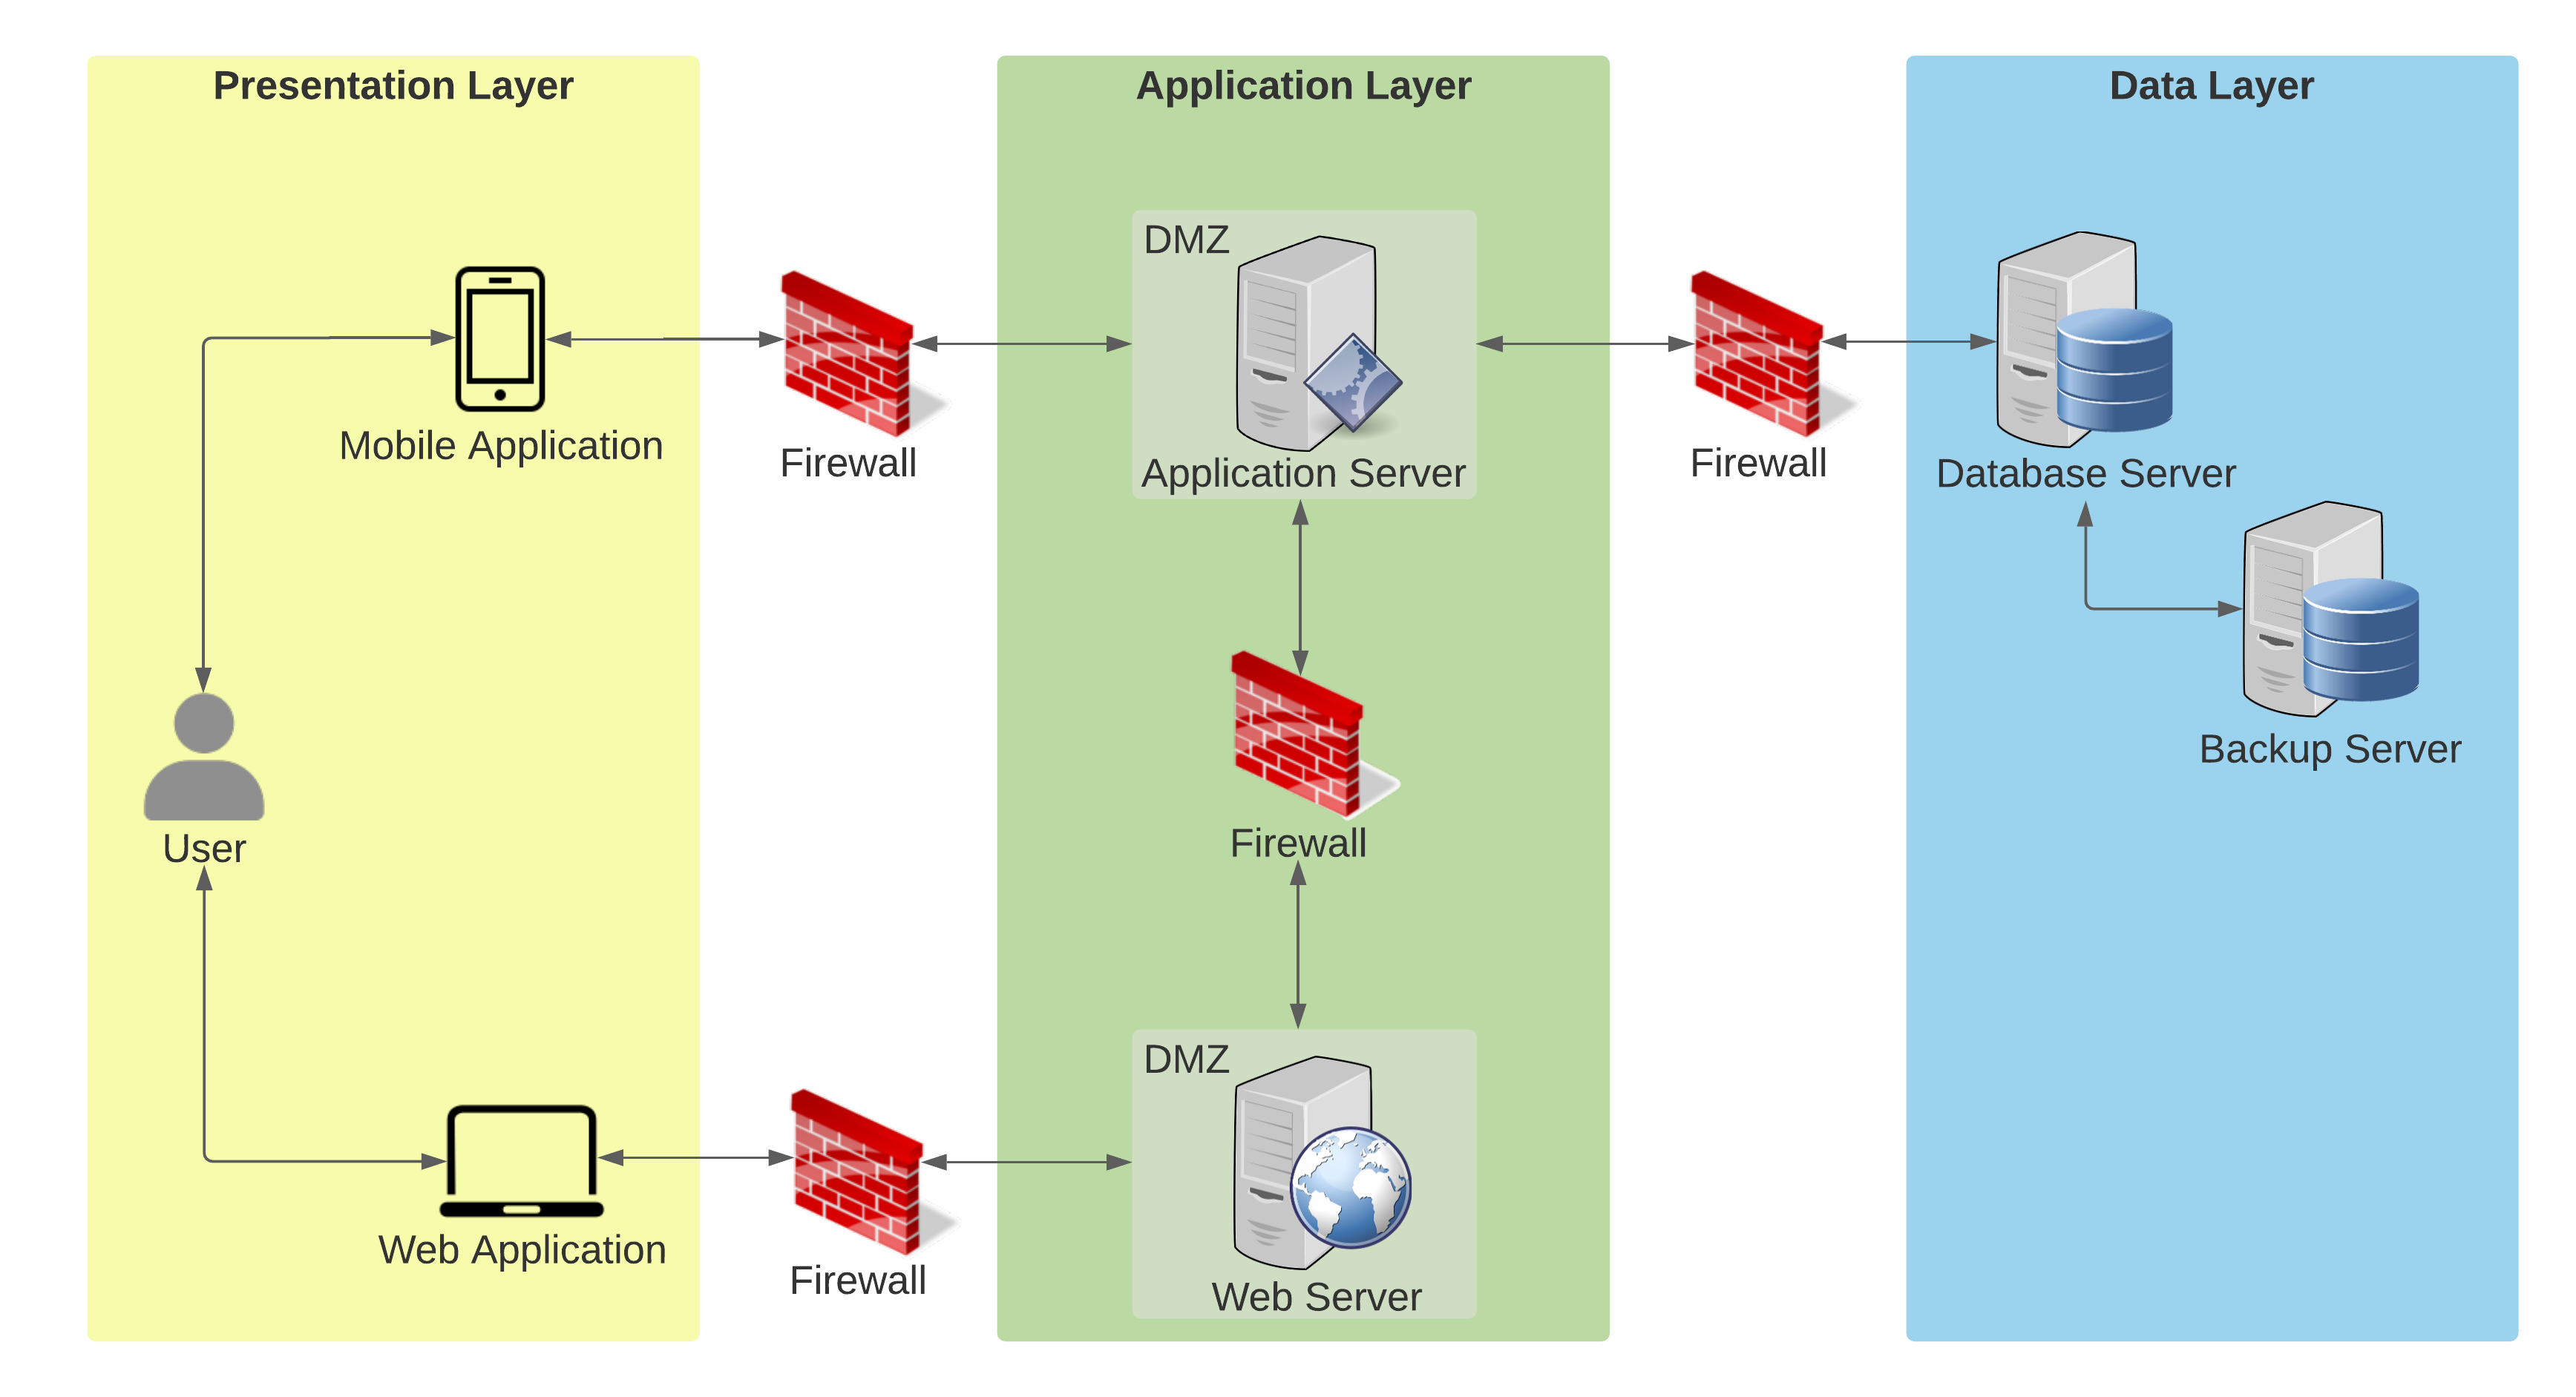
\includegraphics[width=\textwidth,height=\textheight,keepaspectratio]{./Images/System Architecture.png}
  \caption{System Architecture}
\end{figure}
\end{center}

The Application Server is the core of the system’s architecture as it is the central point between all the other components. It holds the business logic of the system with Web Server. Web and Application servers communicate to each other. It has persistent connection with Data tier and by communicating with its DBMS it can handle all the operations of reading, writing and uploading of data.\\

The service is supposed to be accessed through both a web application and a mobile application, and this is valid for all kinds of users. Users who access through DREAM web application can communicate with the Web Server while users logged into the mobile application communicate directly with the Application Server.\\

To guarantee high level of security due to the sensitivity of treated data, firewalls are installed.\\
Specifically, there are firewalls between the Internet accessed by the customer to use the application and the Web Server and between the latter and the Application Server in order to create a demilitarized zone (DMZ), so that the external network can access only to the resources exposed in the DMZ. \\
In order to ensure secure access to the database and to delimit the internal network (IN), a firewall is placed between the Application Server and the Database Server.\\
Moreover, the Database Server periodically stores critical data in the Backup Server. \\

The described architecture has been chosen because tiering ensures the ability to scale applications, guaranteeing the system scalability and flexibility to future integrations and modifications.
The servers that constitute each tier in fact may differ both in capability and number. If needed, it can be possible to add more servers (horizontal scaling or scaling out) or more powerful servers (vertical scaling or scaling up) to each singular tier.  

\subsection{Class Diagram}
In the RASD document a Class Diagram has been showed to model the problem, including all the entities involved without going into too much detail.\\
For this reason, in this section an updated Class Diagram is introduced to represent the system from an  implementation oriented point of view. \\

The following diagram differs from the one presented in the RASD in two aspects:
\begin{itemize}
    \item the main methods of each kind of user are presented;
    \item all attributes' data types are specified.
\end{itemize}

\begin{figure}[H]
  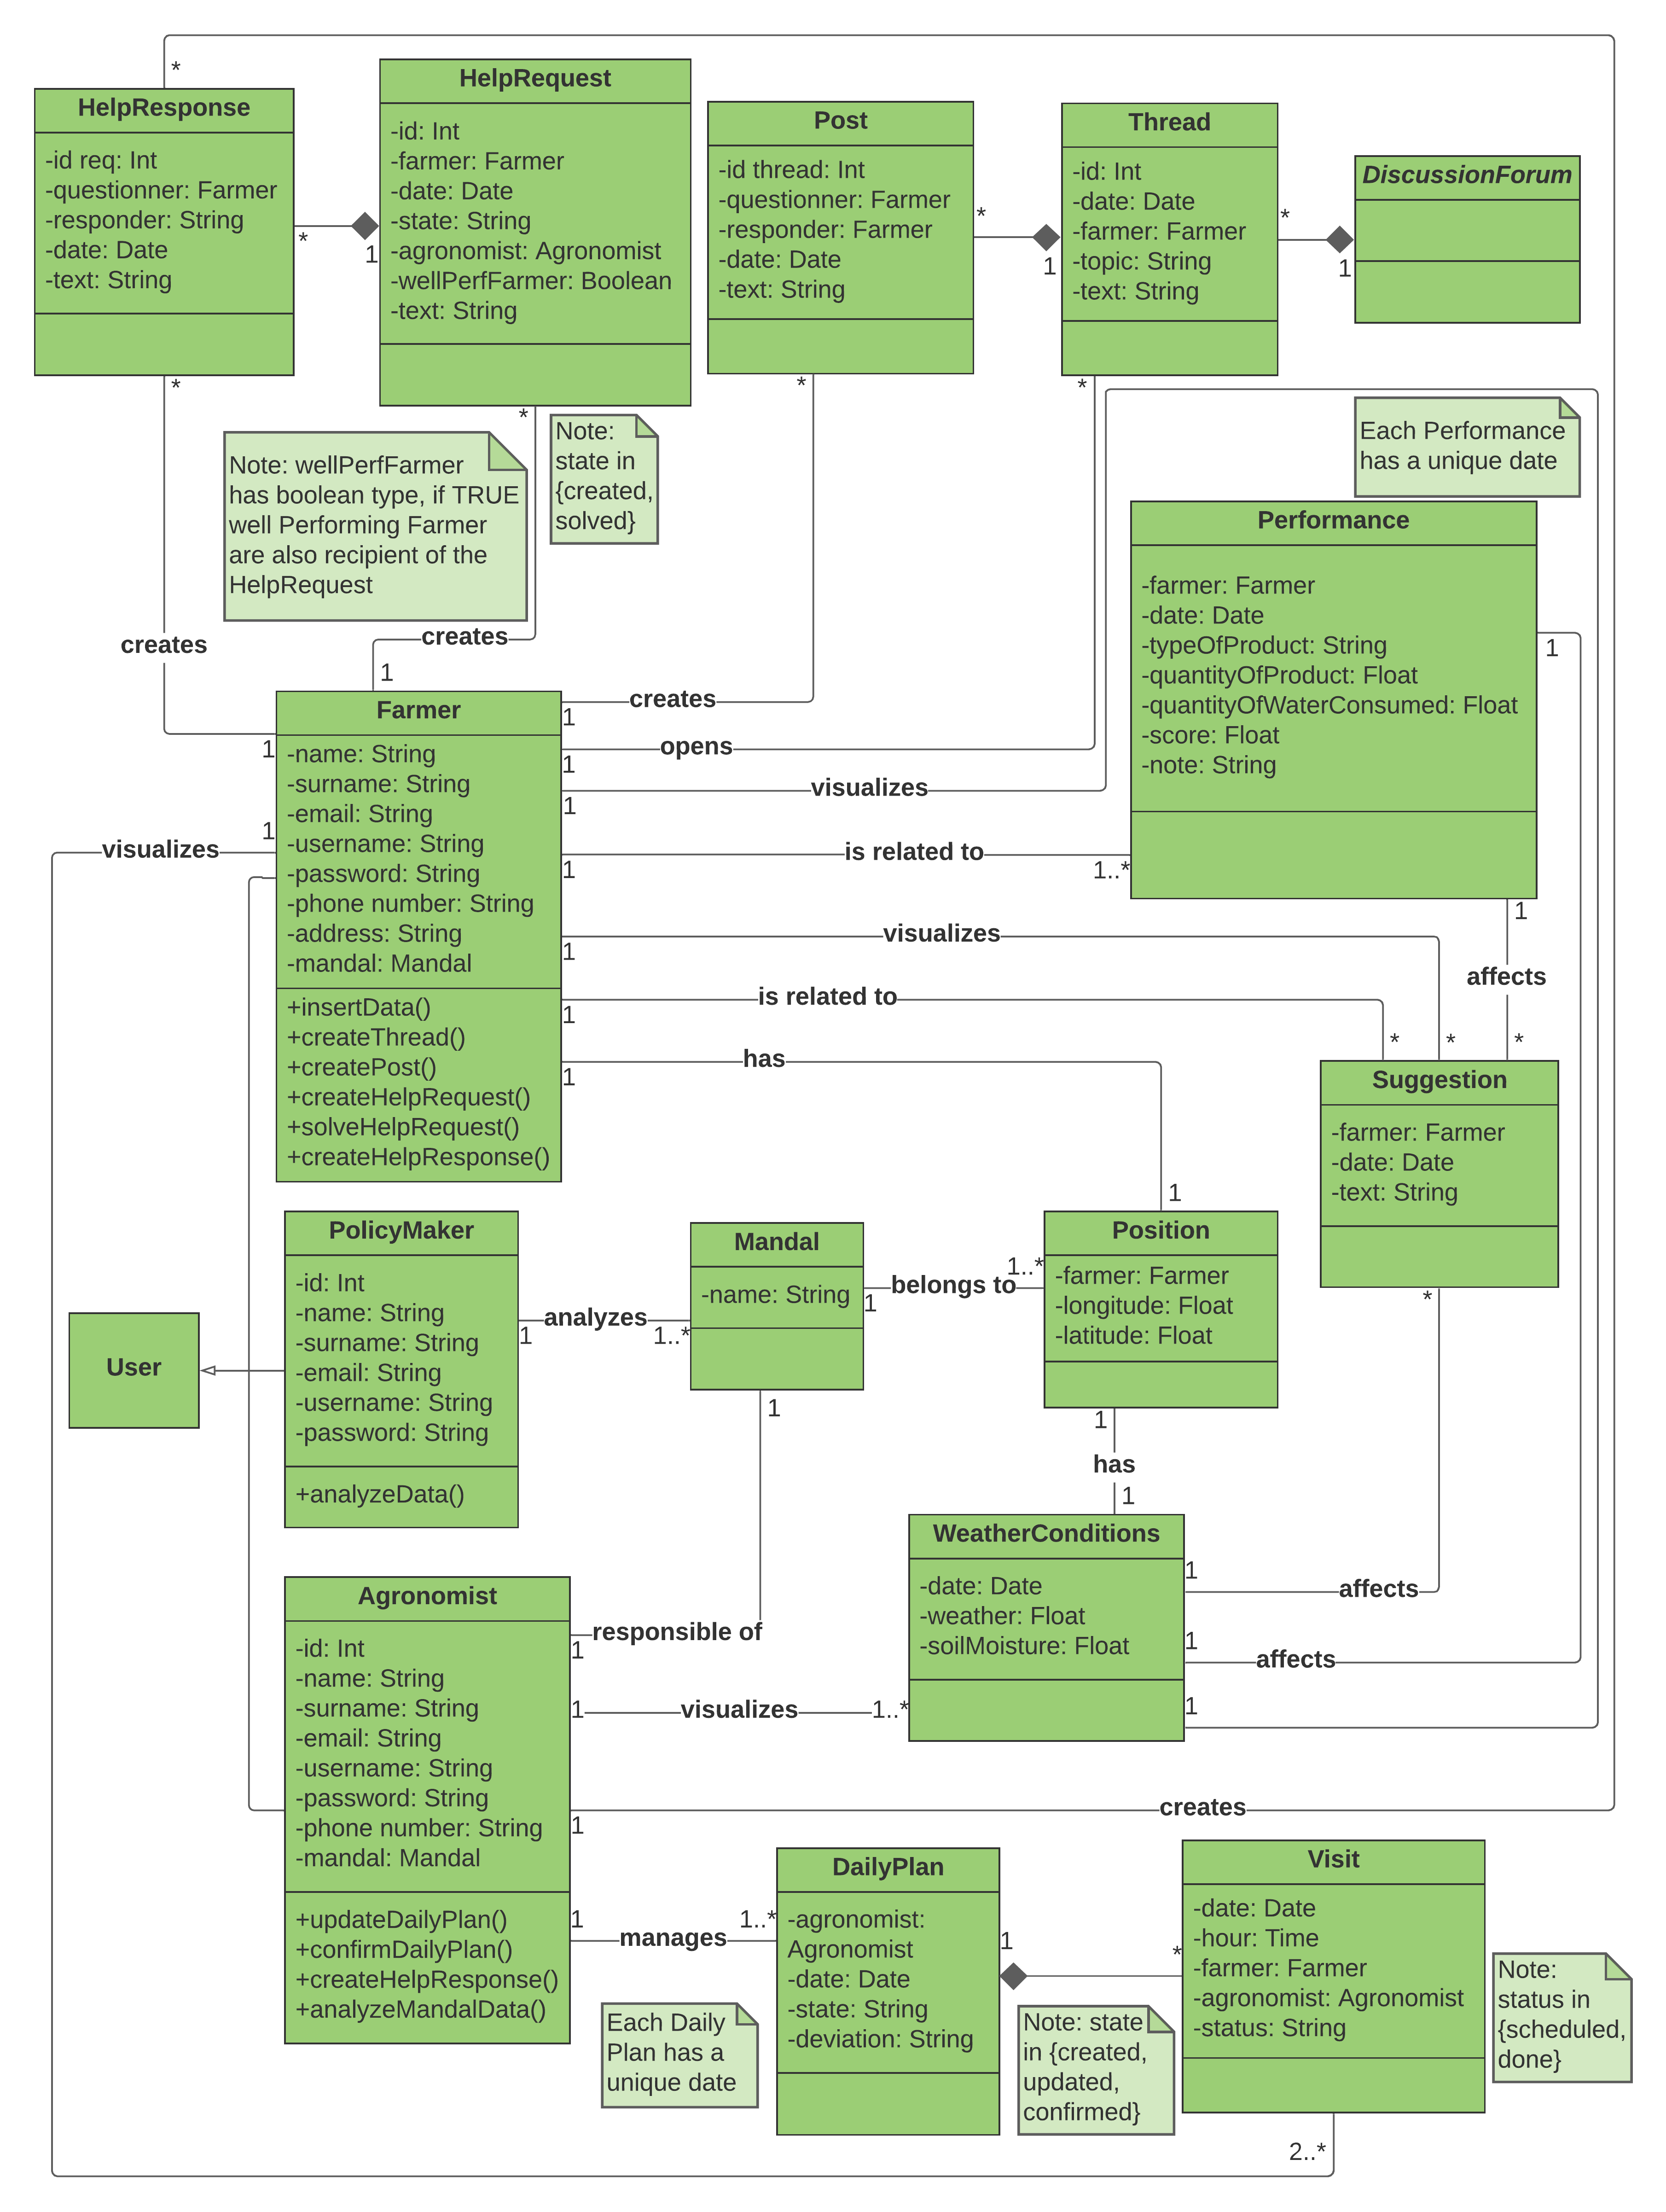
\includegraphics[width=125.5mm,scale=0.9]{./Images/Class Diagram.png}
  \caption{Class Diagram}
\end{figure}

\newpage
\section{Component View}
The purpose of this section is to show the component diagram which is intended to represent the internal structure of the modeled software system in terms of its main components and the relationships among them.

The following legend is used:
\begin{center}
    \begin{figure}[h!]
  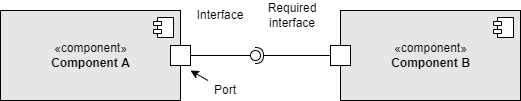
\includegraphics[width=\textwidth,height=\textheight,keepaspectratio]{./Images/Component legend.png}
  \caption{Component legend}
\end{figure}
\end{center}

All components within the diagram are described in detail below.
\begin{itemize}

\item \textbf{WebApplication}: it manages all user interactions with the web application and associates them with the required functions.
It deals with managing all notifications addressed to a specific user.

\item \textbf{MobileApplication}: it manages all user interactions with the mobile application and associates them with the required functions.
It deals with managing all notifications addressed to a specific user.

\item \textbf{AuthenticationService}: it is a service that is involved when login is performed (both from the mobile app and the web app). It checks user permissions according to the role she/he has.
In order to verify the credentials inserted by the user, this component is directly connected with DatabaseAccess component. 

\item \textbf{RegistrationService}: it manages the registration of a unregistered user; in particular, it allows to retrieve farmer's position thanks to the connection to GoogleMapsAPI component. It also accesses the database managed by the Telangana government to check the validity of the ID code entered by the policy maker and agronomist during registration in DREAM. Access to this database takes place thanks to the TelanganaGovernmentService component.
In order to store the new user in the database, the component must be connected to the DatabaseAccess component. 
RegistrationService component includes the following subcomponent.

\begin{itemize}

\item \textbf{EmailManager}: it is necessary when a user who has not yet registered wants to register. To verify his/her email during registration, the system automatically sends a confirmation email to the user and activates a 10-minute timer within which the user must confirm his/her registration.
\end{itemize}
\item \textbf{PolicyMakerService}: This component includes the following subcomponents.

\begin{itemize}
    \item \textbf{TimeChartService}: it computes and displays Telangana’s farmers data in a graph so that the policy maker can analyze the various parameters of interest over time.  In order to collect all the data of interest, the component must be connected to the DatabaseAccess component. 
    \item \textbf{MapService}: it computes and displays Telangana’s farmers performance map using some filters. In order to collect all the data of interest, the component must be connected to the DatabaseAccess component. The connection to GoogleMapsAPI component allows to process the map to be displayed. 
\end{itemize}

\item \textbf{AgronomistService}: This component includes the following subcomponents.

\begin{itemize}
    \item \textbf{HelpResponseService}: it allows an agronomist to manage the response to a help request received. In order to retrieve all the help requests with a certain agronomist as a recipient and store the new help response created by him/her, the component must be connected to the DatabaseAccess component. 
    \item \textbf{MandalMapService}: it retrieves and displays relevant personal data of farmers and their performance score on the map of a mandal. This component is closely linked to the TableService component, which is called up as soon as the agronomist selects a farmer of interest on the map. Obviously, in order to collect all the data of interest, the component must be connected to the DatabaseAccess component. 
    The connection to GoogleMapsAPI component allows to process the map to be displayed.
    \item \textbf{TableService}: it retrieves and displays the table of farmers’ performance in descending order based on their performance score. Obviously, in order to collect all the data of interest, the component must be connected to the DatabaseAccess component.
    \item \textbf{DailyPlanService}: it deals with the creation and updating and confirmation of the daily plan of a agronomist. Specifically, it guarantees that for each farmer there are at least two visits per year by the responsible agronomist. To retrieve the scheduled plan, this component must be connected with DatabaseAccess component.
    \item \textbf{WeatherForecastsService}: it collects the data related to the weather forecasts in the mandal of a certain agronomist according to the date selected by the agronomist. To retrieve weather forecasts, it needs to be connected to the external API TelanganaGovernmentService component. 
    The connection to CopernicusClimateDataStoreService component allows to retrieve soil moisture in the mandal.
    These data are placed on the appropriate mandal map thanks to an external API component: GoogleMapsAPI.
\end{itemize}

\item \textbf{FarmerService}: This component includes the following subcomponents.

\begin{itemize}
    \item \textbf{HelpRequestService}: it is necessary for the creation and subsequent management of help requests by the farmer. The connection to DatabaseAccess component allows it to retrieve the recipients to whom the request can be sent (agronomist in charge of the mandal and well performing farmers).\\
    In addition, if a (well performing) farmer has received a help request from another farmer, this component takes care of managing the function that allows the farmer to respond to the request.
    \item \textbf{DiscussionForumService}: it manages the creation of threads by a farmer on the discussion forum, the creation of posts in response to a specific thread (always by other farmers) and the search by topic of a thread already created. It also performs these functions thanks to the connection to the DatabaseAccess component.
    \item \textbf{VisitService}: it retrieves the visits scheduled for a farmer that corresponds to the daily plan of an agronomist.
    Since visits are stored in the database, to retrieve them, this component must be connected to the DatabaseAccess component.
    \item \textbf{PerformanceService}: it takes care of updating a farmer's performance data every time he/she enters new data about his/her crop. It is connected to the DatabaseAccess component not only to store the computed performance but also to get farmer's position and his/her last performance date (to take into account the right time interval for which performance has to be computed).
    It also is connected to external API TelanganaWaterIrrigationService to compute the quantity of water consumed. Furthermore it is linked to WeatherConditionService component which allows to retrieve weather conditions and soil moisture.
    \item \textbf{WeatherConditionService}: it collects the data related to weather conditions based on the farmer's position. To accomplish this task, it needs to be connected to the external API TelanganaGovernmentService as well as to the CopernicusClimateDataStoreService component. It also has to be connected to DatabaseAccess component to retrieve farmer's position.
    \item \textbf{SuggestionsService}: it is used to elaborate farmer's suggestions based on his/her relevant information regarding his/her production and the position of his/her farm. These data are obtained thanks to the connection to the DatabaseAccess and WeatherConditionService components.
\end{itemize}

\item \textbf{DatabaseAccess}: it is responsible to retrieve (and store) data from (to) a data source. In this case, it manages the access to the database.

\item \textbf{Database}: This component includes the following subcomponent.

\begin{itemize}
    \item \textbf{DBMS}: Database Management System refers to a software that allow users to access databases and manipulate, maintain, report, and relate data. It is used to reduce data redundancy, share data in a controlled manner, and reduce data integrity issues.
\end{itemize}

\item \textbf{ExternalAPIs}: This component includes the following subcomponents.

\begin{itemize}
    \item \textbf{GoogleMapsAPI}: it allows the connection of the application to Google Maps APIs. All functions that require access to geographical data, not yet saved in the internal database, will rely on this component.
    \item \textbf{CopernicusClimateDataStoreService}: it is responsible for retrieving soil moisture data in the Telangana region.
    \item \textbf{TelanganaGovernmentService}: it takes care of retrieving data relating to weather conditions in Telangana region. It also used to access ID codes' DB managed by Telangana government to check validity of ID code inserted by policy makers and agronomist while registering into DREAM. 
    \item \textbf{TelanganaWaterIrrigationService}: it is responsible for retrieving the amount of water consumed by each farmer in the Telangana region.
\end{itemize}

\end{itemize}


\def\fillandplacepagenumber{%
 \par\pagestyle{empty}%
\vbox to 0pt{\vss}\vfill
\vbox to 0pt{\baselineskip0pt
   \hbox to\linewidth{\hss}%
   \setlength{\footskip}{70pt}
   \baselineskip\footskip
   \hbox to\linewidth{%
     \hfil\thepage\hfil}\vss}}

\begin{landscape}
\begin{figure}[h]
\vspace*{-2cm}
\noindent
\centering
\centerline{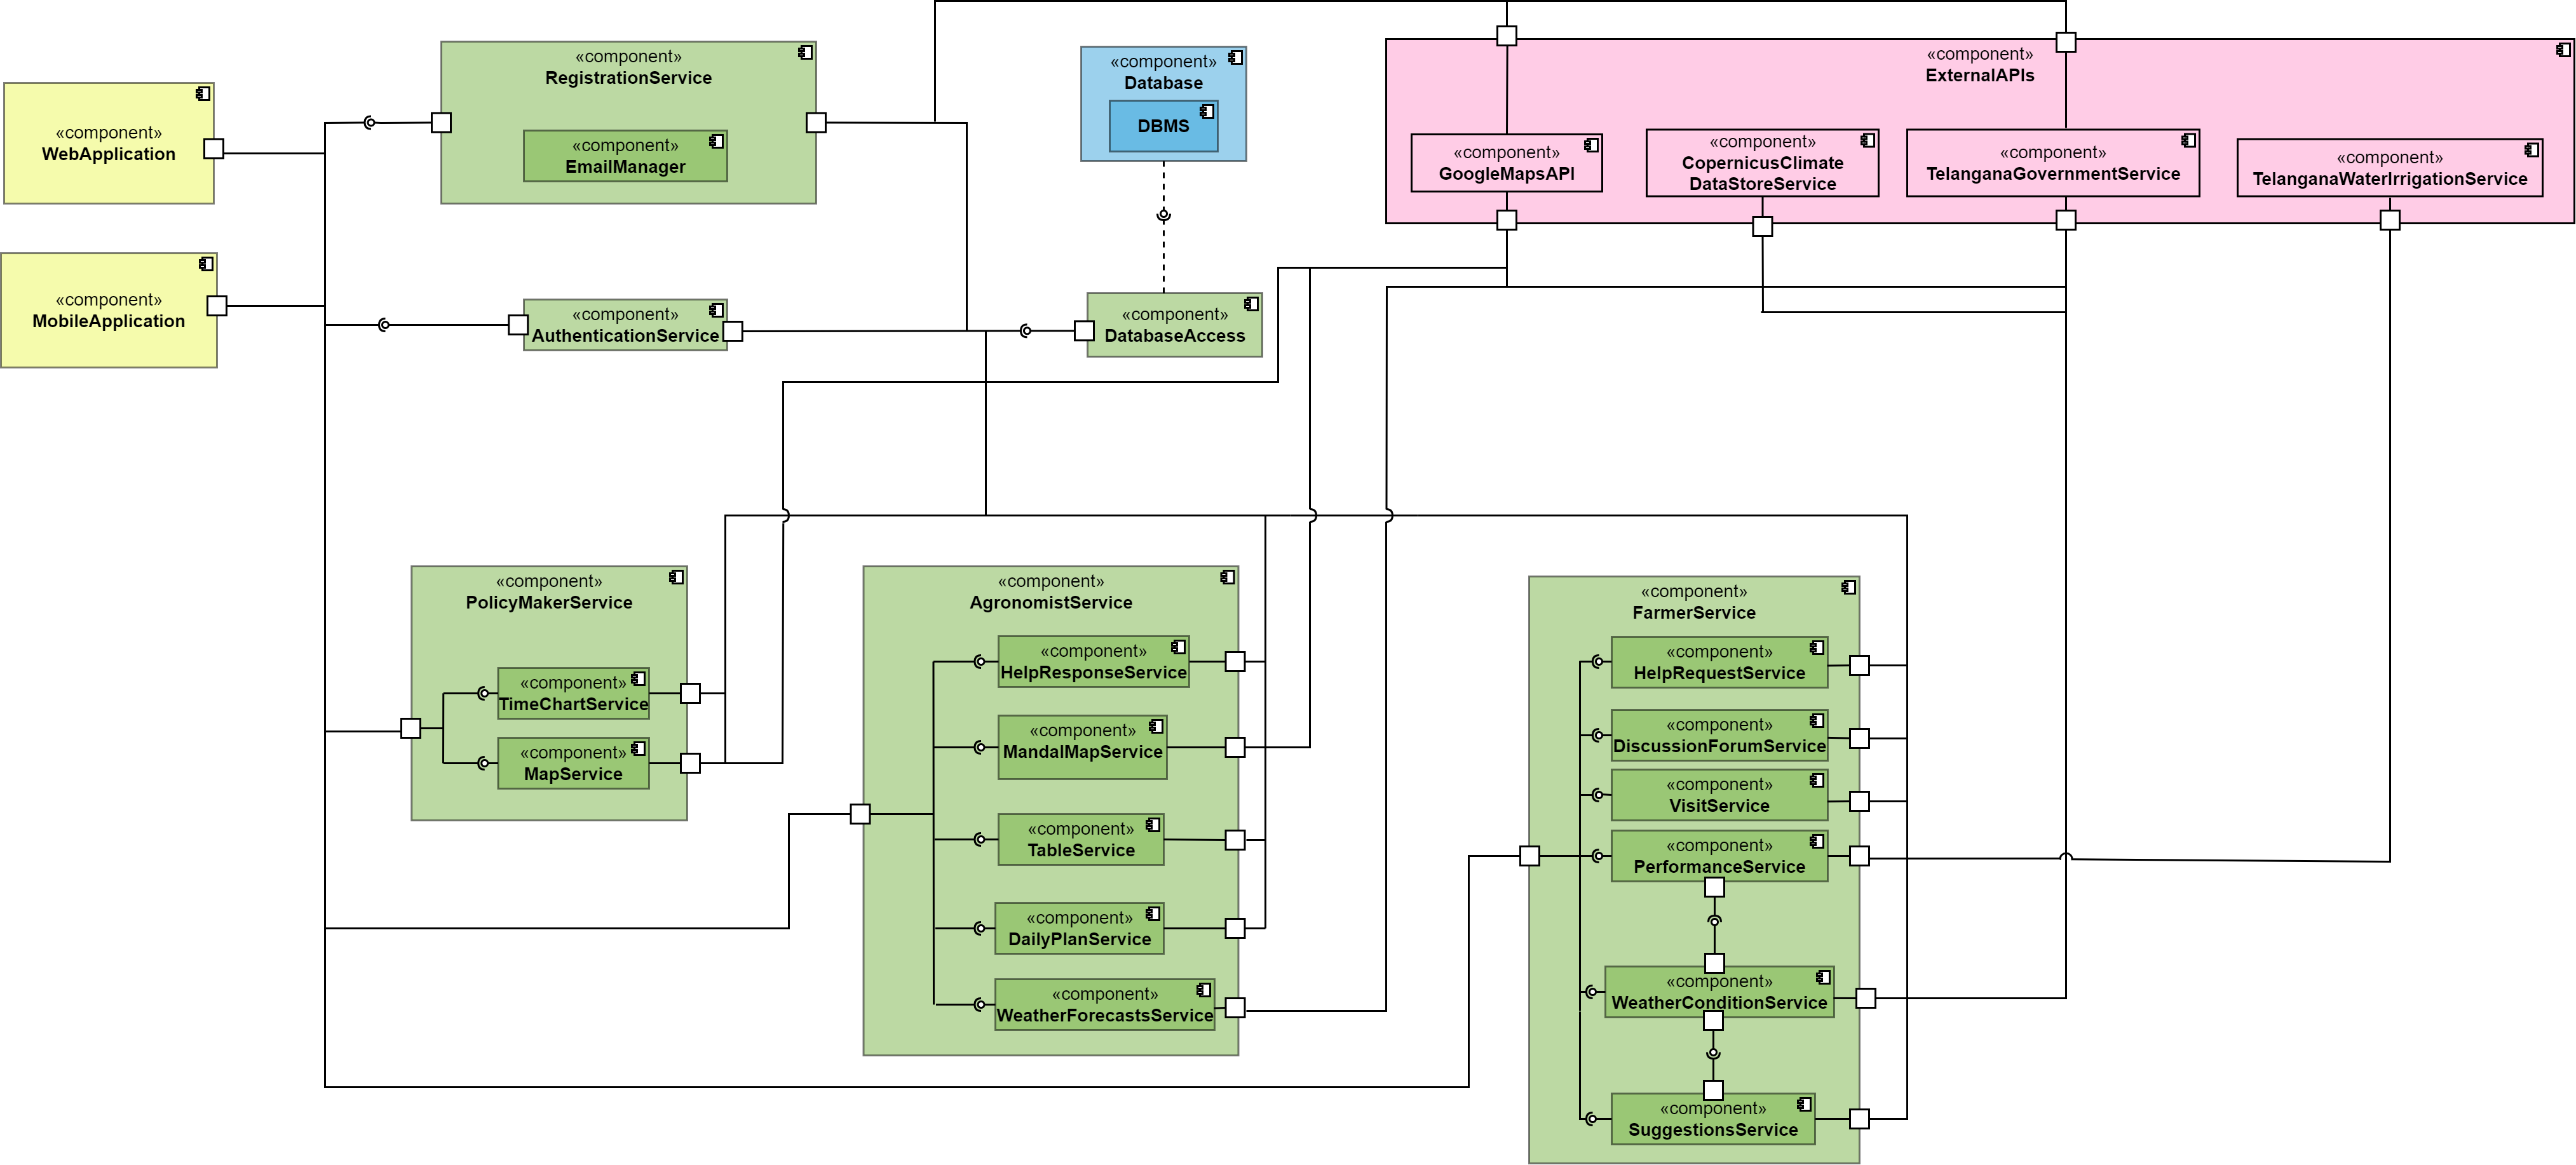
\includegraphics[scale = 0.2]{./Images/Component diagram.png}}
    \caption{Component diagram}
    \vspace*{-12cm}
\end{figure}
\fillandplacepagenumber
\end{landscape}


\section{Deployment View}
This section shows the physical distribution of the system, that is, the environment in which the system runs. Specifically, \textit{Figure 2.4} shows the structure of the hardware components that execute the software.

Firewalls are inserted to ensure security between the different zones and load balancers are designed to distribute the workload.\\

As previously mentioned, the system is divided into 4 Tier, the components of which are described below:
\begin{itemize}
    \item \textbf{Client Tier}: it consists of the client programs used to exploit system services and the devices on which these programs are installed.
    \begin{itemize}
        \item \textbf{Smartphone}: users access the DREAM system and use the related services through a mobile application from a smartphone.
        \item \textbf{Personal Computer}: users access the DREAM system and use the related services through the Web browser from a personal computer.
    \end{itemize}
    \item \textbf{Web Tier}: it consists of components that handle the interaction between client tier and the business tier.  It contains the Web Server.
    \begin{itemize}
        \item \textbf{Web Server}: it provides content to the Web using the HTTP(S) protocol. It mainly works to serve the requested web pages continuously and without interruption. As long as the Web Server is up and running, the corresponding web pages and sites will be available to users on the network.
    \end{itemize}
    \item \textbf{Business Tier}: it processes all dynamic content and the interactions between the Client/Web Tier and the Data tier. It contains the Application Server.
    \begin{itemize}
        \item \textbf{Application Server}: it hosts and exposes business logic and processes. It provides the infrastructure and logical capabilities to support, develop and run applications in a distributed context. The Application Server communicates directly with the Mobile Application through HTTPS protocol, in order to create a lightweight API to request only the necessary data. The Application Server will receive this call, make the call to the external service, filter it, and return only what the application has requested.  This will reduce the amount of data transiting over mobile Internet and thus increase application performance.
    \end{itemize}
    \item \textbf{Data Tier}: it runs the DBMS and holds all of the sensitive application data. It contains database servers.
    \begin{itemize}
        \item \textbf{Database Server}: it allows access to one or more Database Systems and is an essential support for Web Servers in managing the delivery and storage of data. It communicates with the Application Server via the standard TCP/IP protocol and provides access to the physical database which is in charge of storing all persistent data of users who use DREAM.
    \end{itemize}
\end{itemize}\\


\textbf{Firewalls} are also included in the system architecture to delimit safe areas within the system. 
Specifically, there are firewalls between the Internet accessed by the customer to use the application and the Web Server and between the latter and the Application Server in order to create a demilitarized zone (DMZ). The purpose of the DMZ is to add an additional level of security to an internal network, where a node belonging to an external network can only access the services made available, without putting at risk and compromising the security of the entire network.
In order to ensure secure access to the database and to delimit the internal network (IN), a firewall is placed between the Application Server and the Database Server.\\


In order to distribute the load of the requests to the DREAM website among several servers, \textbf{load balancers} are introduced for the Web Server. In this way, the reliability and scalability of the entire architecture increases because requests will be shared equally among the different servers. If one of the servers is unable to respond to the request, the user can still use the service based on one of the active servers.
Similarly, the Web Server may need to query the database to generate responses. Web Servers send database queries to the load balancer which balances the inbound database workload on the database servers.



\def\fillandplacepagenumber{%
 \par\pagestyle{empty}%
\vbox to 0pt{\vss}\vfill
\vbox to 0pt{\baselineskip0pt
   \hbox to\linewidth{\hss}%
   \setlength{\footskip}{70pt}
   \baselineskip\footskip
   \hbox to\linewidth{%
     \hfil\thepage\hfil}\vss}}

\begin{landscape}
\begin{figure}[h]
\vspace*{-2cm}
\noindent
\centering
\centerline{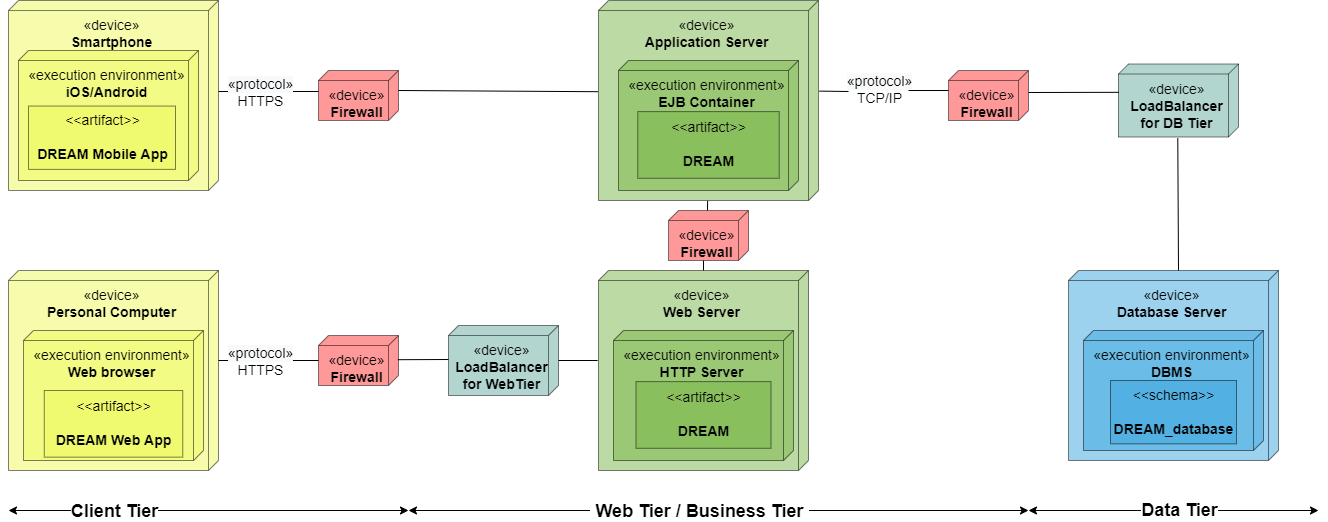
\includegraphics[scale = 0.6]{./Images/Deployment diagram.png}}
    \caption{Deployment diagram}
    \vspace*{-12cm}
\end{figure}
\fillandplacepagenumber
\end{landscape}




\section{Runtime View}

To accomplish specific tasks of DREAM the components listed in \textit{Section 2.2} must interact with each other. To describe the type of interactions which occur between one another, in this section are presented the most relevant sequence diagrams.\\
All functionalities described by the following diagrams can be performed through both Web and Mobile application by the users. 


\def\fillandplacepagenumber{%
 \par\pagestyle{empty}%
\vbox to 0pt{\vss}\vfill
\vbox to 0pt{\baselineskip0pt
   \hbox to\linewidth{\hss}%
   \setlength{\footskip}{70pt}
   \baselineskip\footskip
   \hbox to\linewidth{%
     \hfil\thepage\hfil}\vss}}

\subsection{Farmer registers}

In this sequence diagram it is shown the process of registration attended by the farmer. It is supposed that the farmer has already selected is role in the registration form and the Web/Mobile Application shows him/her the related fields.\\ 
After having switched from the \textit{login} page to the \textit{registration} one, he/she signs up filling in the registration form. Then, Web/MobileApplication checks that all the credentials inserted by the farmer are valid. Then, the registration request is sent from Web/MobileApplication to RegistrationService component which is in charge of retrieving position and mandal of the farmer (through GoogleMapsAPI) before storing his/her data persistently in the Database. Eventually, DatabaseAccess component is called to store the information in the Database. The result of the operation is propagated back to Web/Mobile Application, following in reverse order the same path as before. If the result is negative the registration should be repeated and an alert regarding registration failure is sent to the farmer. If the result is positive the farmer is redirected to a waiting page and the Web/mobile application calls RegistrationService component to send a confirmation email to the farmer. The function is propagated to EmailManager component which is in charge to check if the farmer has clicked on the confirmation link in the email within a certain time limit. The result of the operation is propagated back to Web/MobileApplication, following in reverse order the same path as before. If the result is negative an alert regarding confirmation failure is sent to the farmer and he/her has to request for the generation of a new confirmation email to repeat the process. If the result is positive the farmer is redirected to \textit{login} page.\\
The process of registration is different for the agronomist and the policy maker. In fact, the credentials to be inserted differ in particular in a unique id code which is checked calling an appropriate function to be propagated from Web/MobileApplication to RegistrationService. This component is in charge of verifying the id code calling TelanganaGovernmentService component. Eventually, the result of the operation is returned following in reverse order the same path as before and if it is false the filling operation must be repeated. 

\newpage
\begin{landscape}
\begin{figure}[h]
\vspace*{-2cm}
\noindent
\centering
\centerline{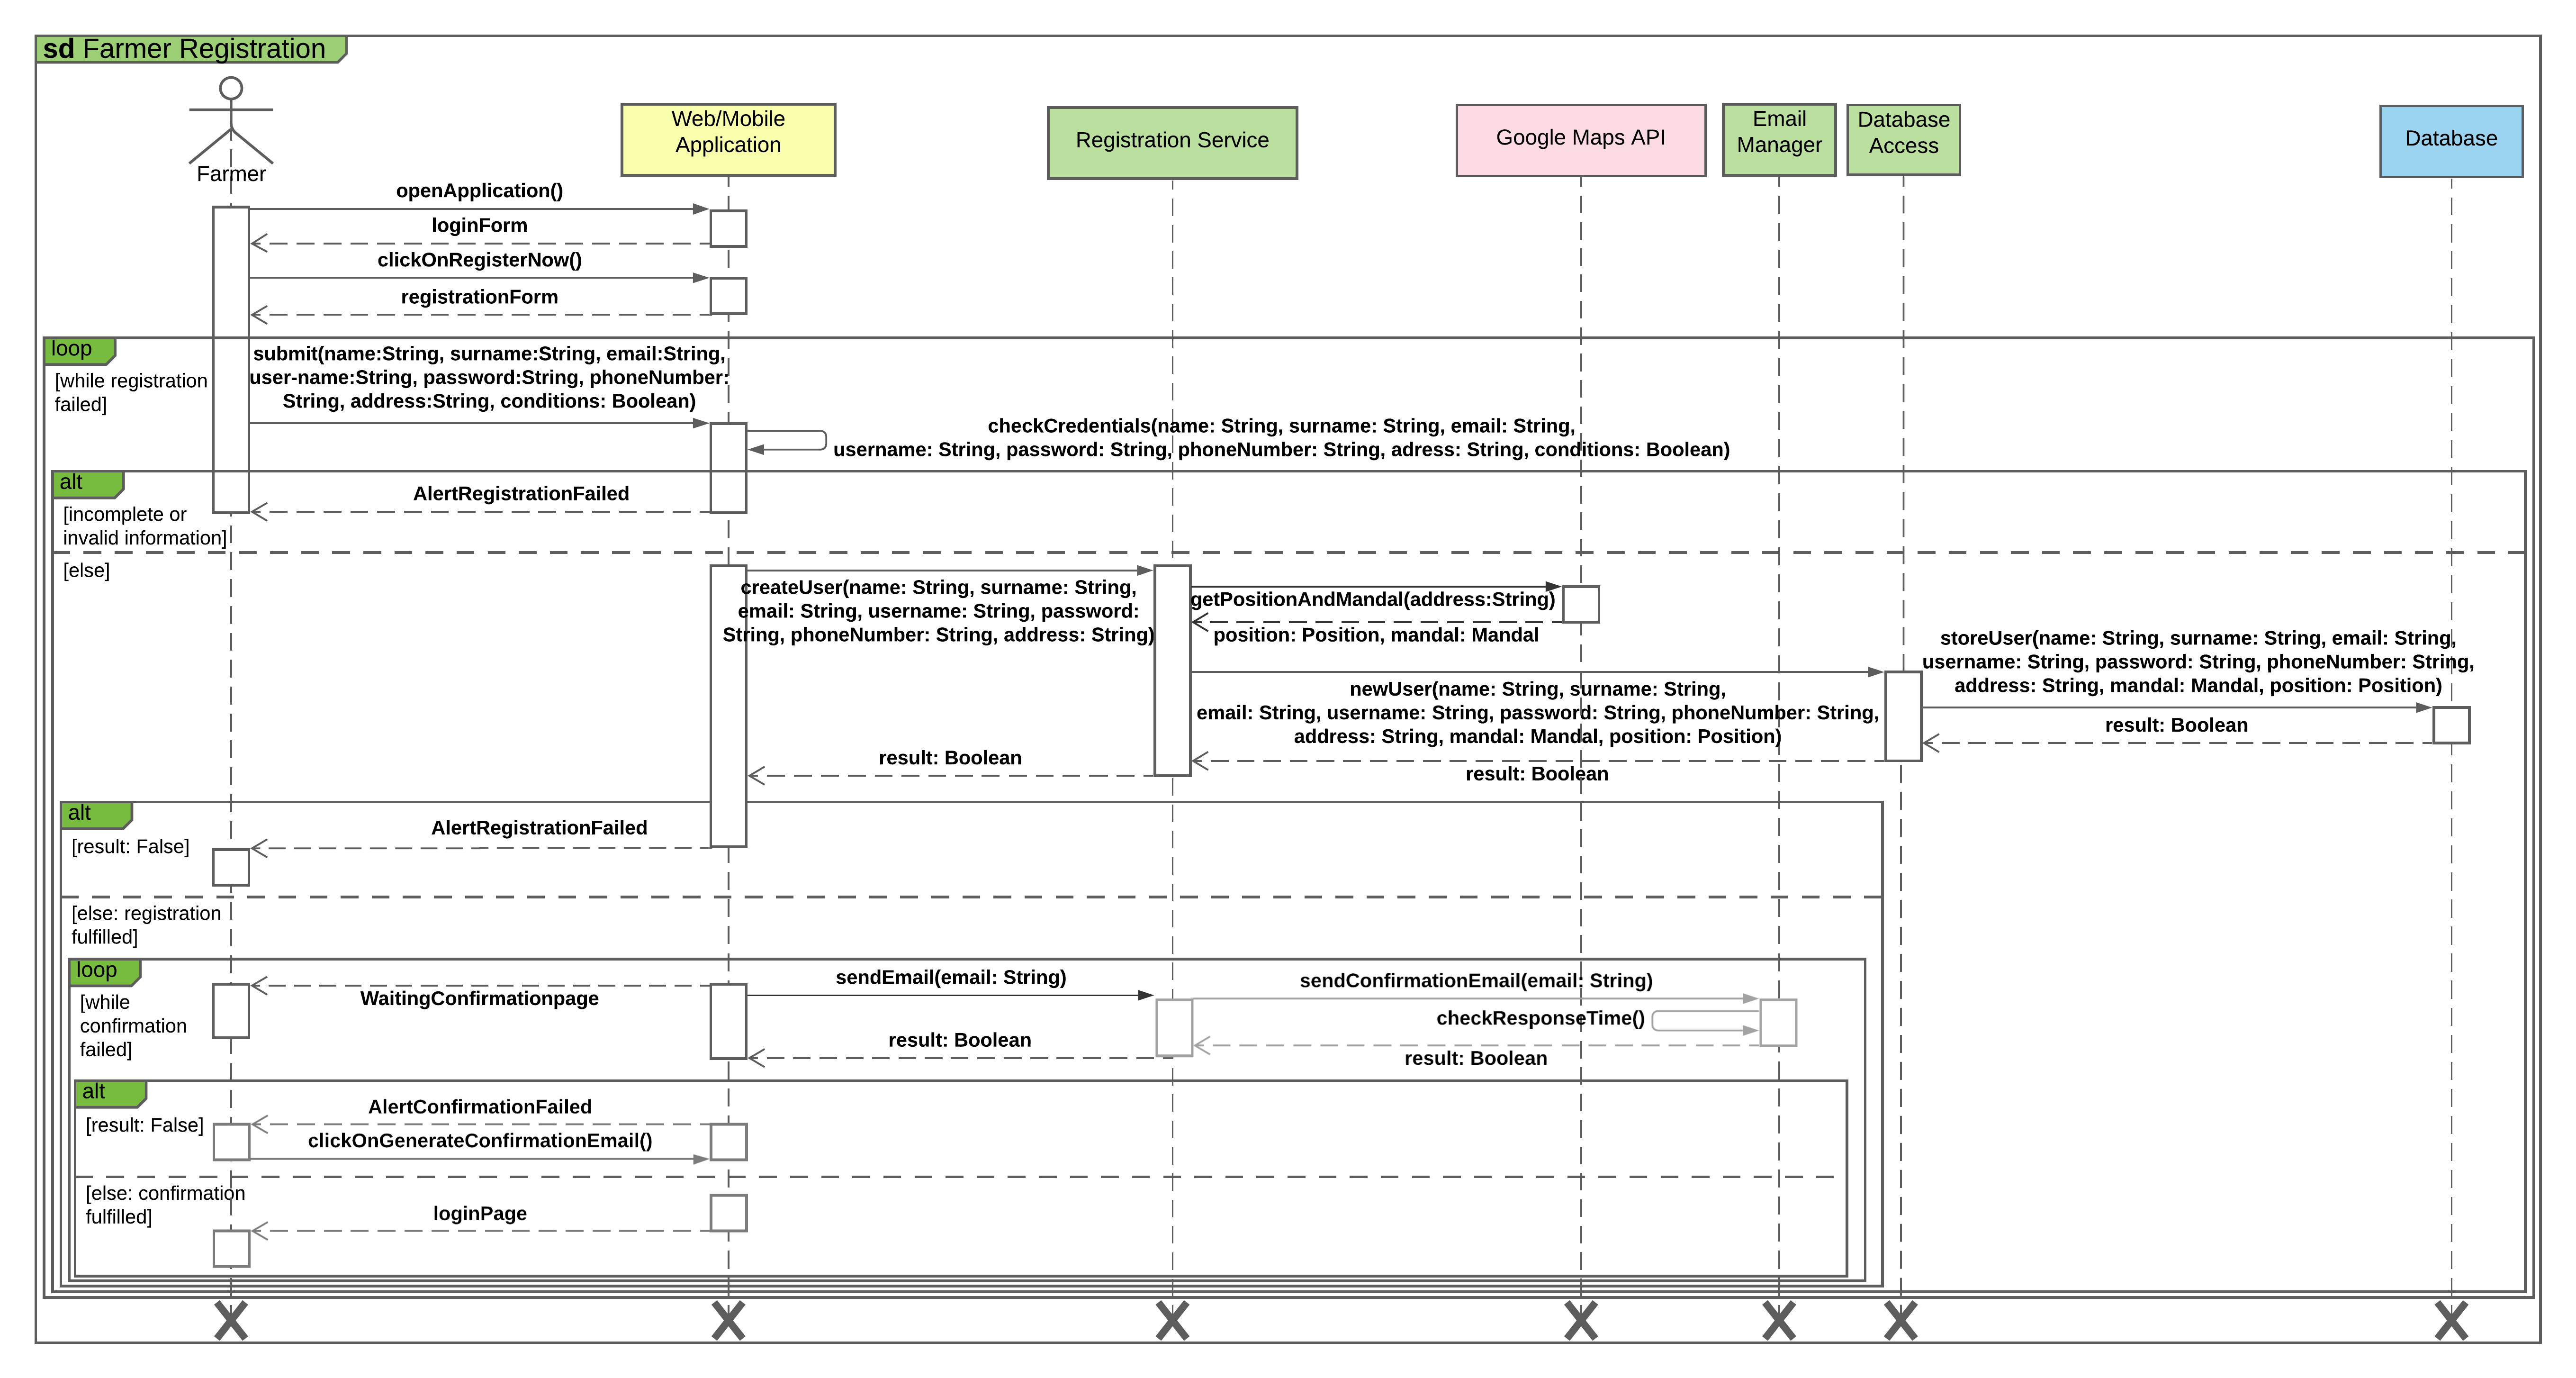
\includegraphics[scale= 0.108]{./Images/Sequence diagram/Farmer Registration Sequence Diagram.png}}
    \caption{Farmer registers}
    \vspace*{-12cm}
\end{figure}
\fillandplacepagenumber
\end{landscape}

\subsection{Farmer logs in}

This sequence diagram shows the login procedure executed by a farmer who is already registered.\\
After having opened DREAM application on his device, the farmer fills in the form with his username and password. The inserted credentials are checked by Web/MobileApplication, which controls whether one or both these two fields are missing. If it is the case, it shows to the farmer an alert regarding the login failure. If credentials are not missing, the AuthenticationService is called to check the validity of credentials and this component propagates the request to the DatabaseAccess that provides access to the Database, where all the users credentials are stored persistently. If a couple of username and password that matches the one inserted by the farmer is found, the login is successfully completed, otherwise an alert is shown and the operation must be repeated. This process is the same for all kind of users. \\
For the sake of completeness, in the sequence diagram it is shown also what is returned to the farmer who has successfully logged in. \\ 
The farmer must be able to visualize his/her \textit{homepage}, in which are reported weather conditions regarding his/her position and his/her next visit scheduled in the daily plan. For this reason a request to get weather conditions is propagated from Web/MobileApplication to WeatherConditionService which is able to retrieve weather and soil moisture from external APIs given the position of the user. The result of the operation is propagated to Web/MobileApplication. Then, the latter component send a request to VisitService. The request is propagated to DatabaseAccess to access the Database and retrieve all visits related to the farmer, which are returned eventually to VisitService, component that gets the next visit among them and returns it to Web/MobileApplication. Eventually, the \textit{homepage} is shown to the farmer. 

\newpage
\begin{landscape}
\begin{figure}[h]
\vspace*{-2cm}
\noindent
\centering
\centerline{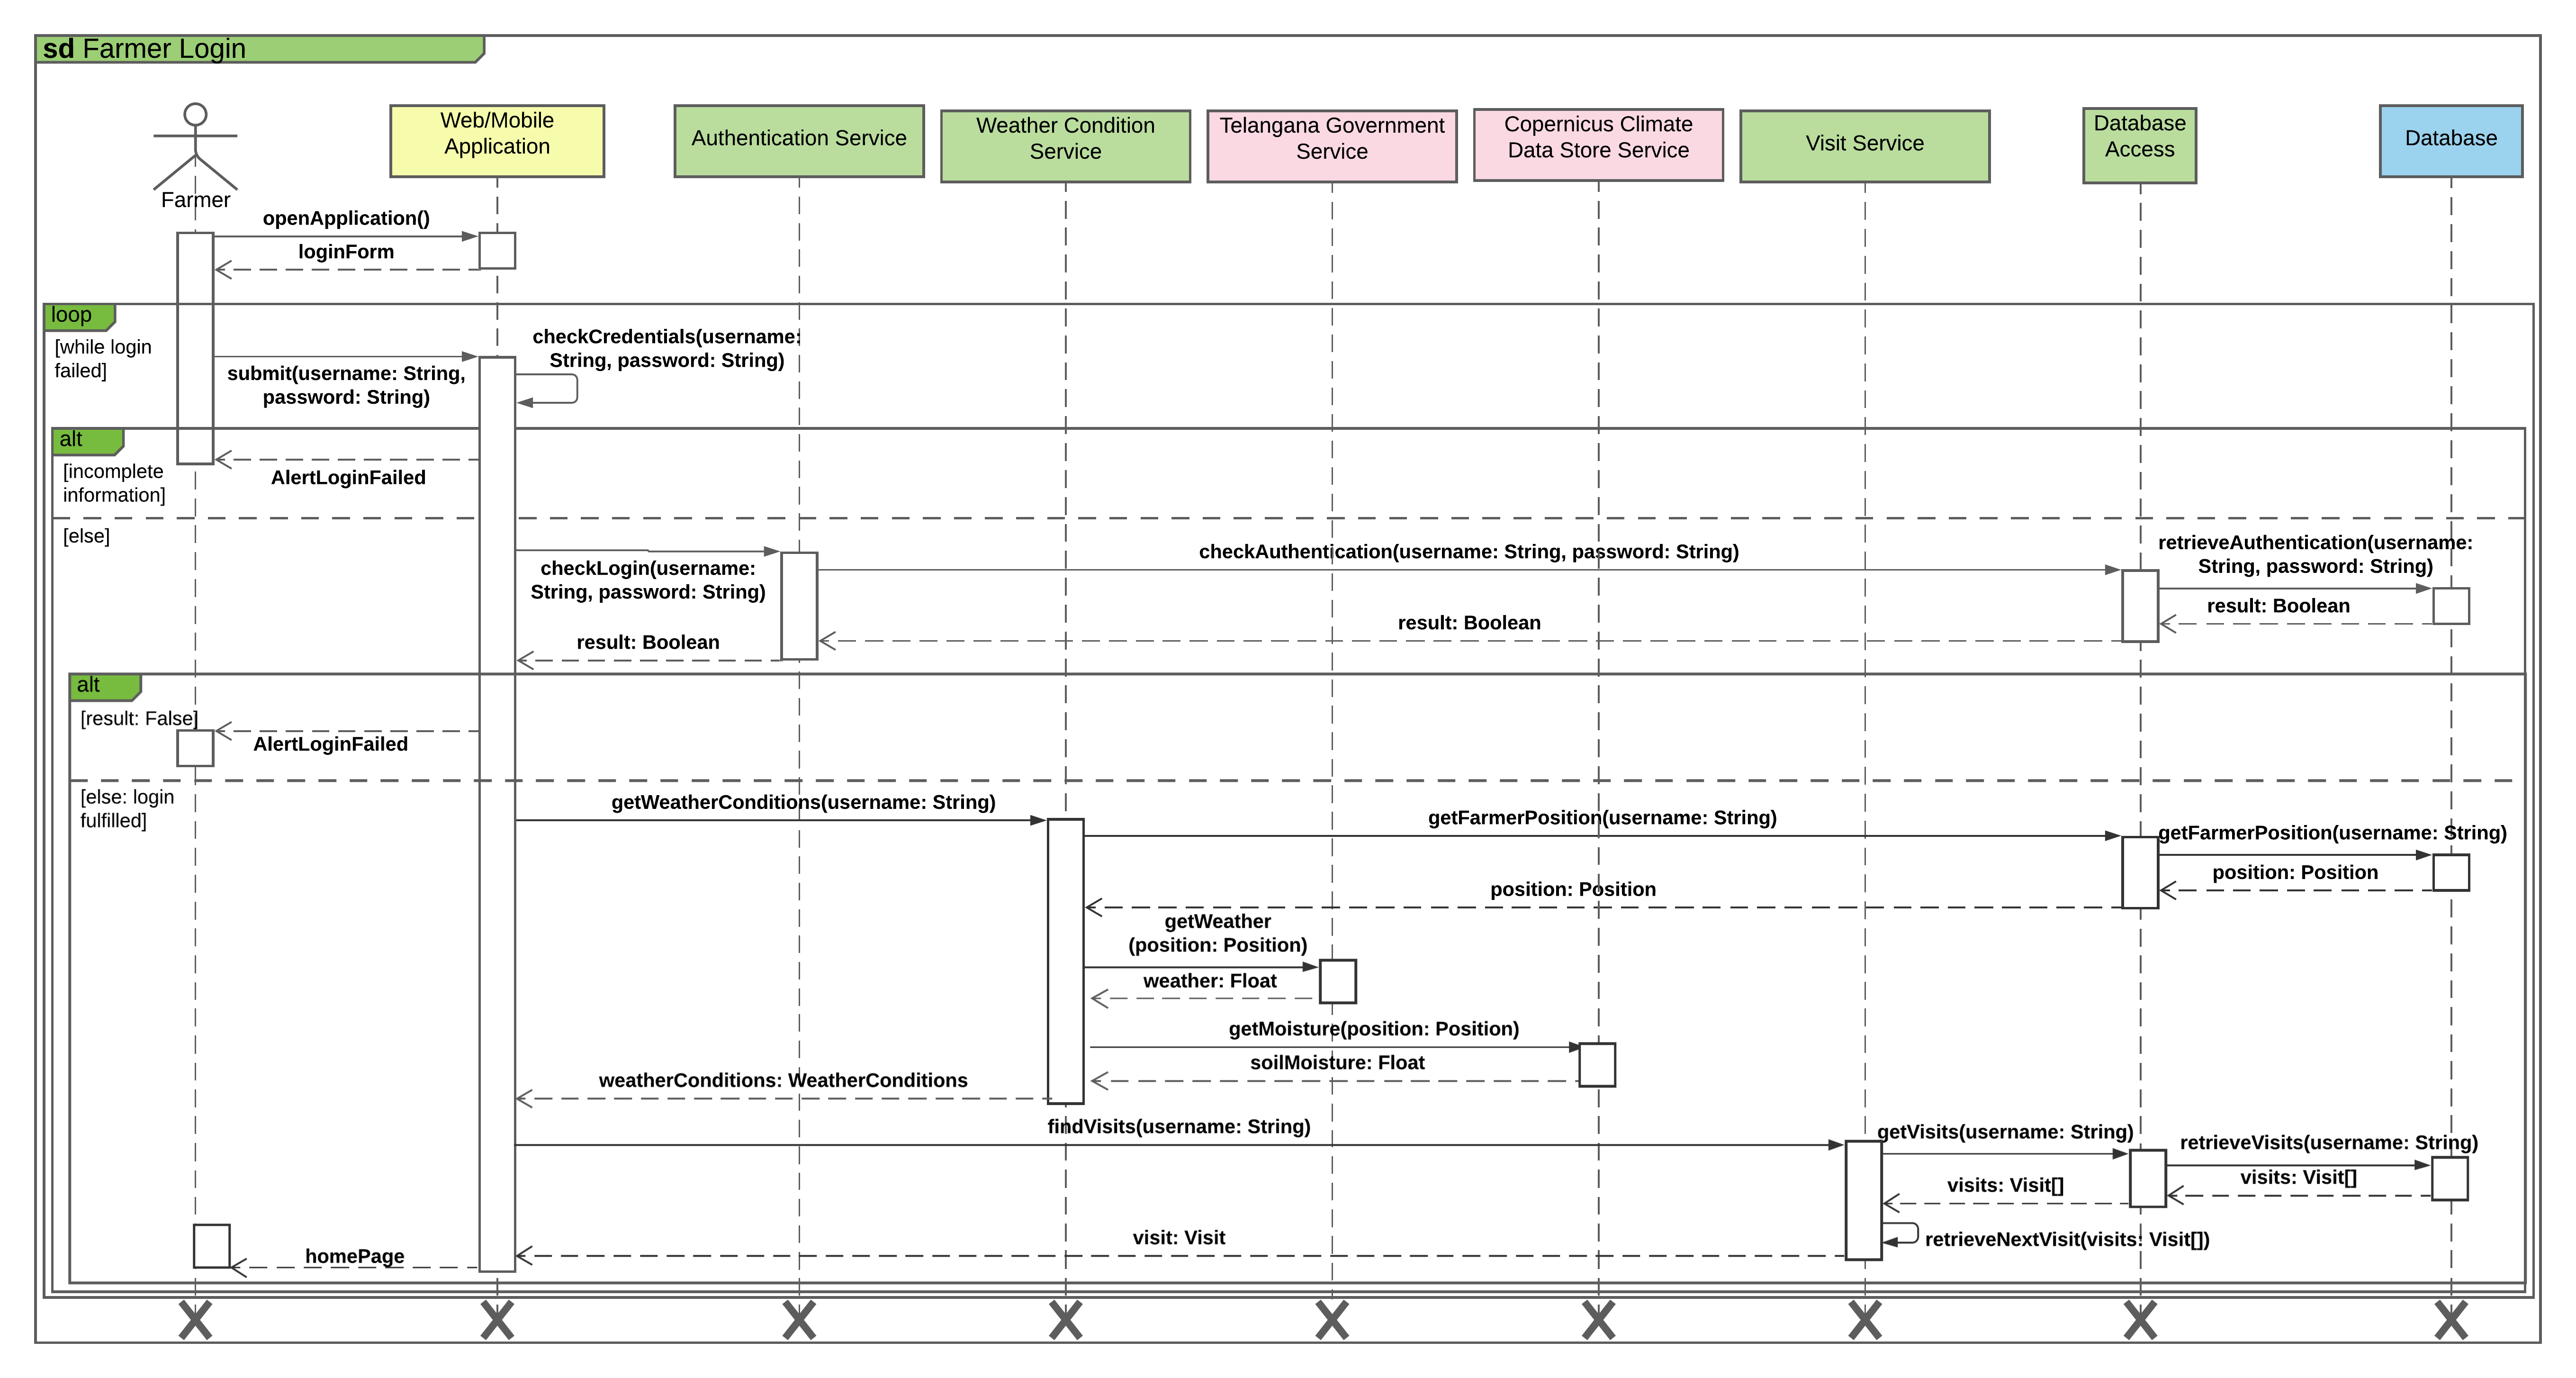
\includegraphics[scale= 0.108]{./Images/Sequence diagram/Farmer Login Sequence Diagram.png}}
    \caption{Farmer logs in}
    \vspace*{-12cm}
\end{figure}
\fillandplacepagenumber
\end{landscape}

\subsection{Farmer inserts data about his/her production}

This sequence diagram shows the procedure of inserting data about production executed by a farmer who is already registered and logged in.\\
After having opened DREAM application on his device, the farmer clicks on \textit{Insert} icon in the homepage. Web/MobileApplication returns a form to be filled in. Once the farmer submits it Web/MobileApplication checks whether fields are missing or invalid. If it is the case, it shows an alert to the farmer. If it is not the case, the PerformanceService is called to compute the performance of the farmer.\\
Farmer's performance score is affected by weather conditions, for this reason it is necessary to retrieve farmer's position and his last performance date to define the time interval for which weather and soil moisture data must be retrieved. PerformanceService calls the DatabaseAccess. Database access provides access to the Database, where all the farmers' performances and positions are stored persistently. Farmer's last performance date and position are retrieved and returned eventually to PerformanceService.\\
The latter component is also able to get quantity of water consumed by the farmer calling TelanganaWaterIrrigationService. The result is returned back and a function is called by PerformanceService to add it to  the data inserted by the farmer. At this moment, two functions are called and propagated to two different external APIs (TelanganaGovernmentService and CopernicusClimateDataStoreService) to retrieve weather and soil moisture.\\ 
PerformanceService has now all necessary data to compute performance score, for which a proper function is called.\\
Eventually, farmer's performance is stored in the Database through a request which is propagated through DatabaseAccess to Database. A result is return following the same path. If it is false the process must be repeated. 

\newpage
\begin{landscape}
\begin{figure}[h]
\vspace*{-2cm}
\noindent
\centering
\centerline{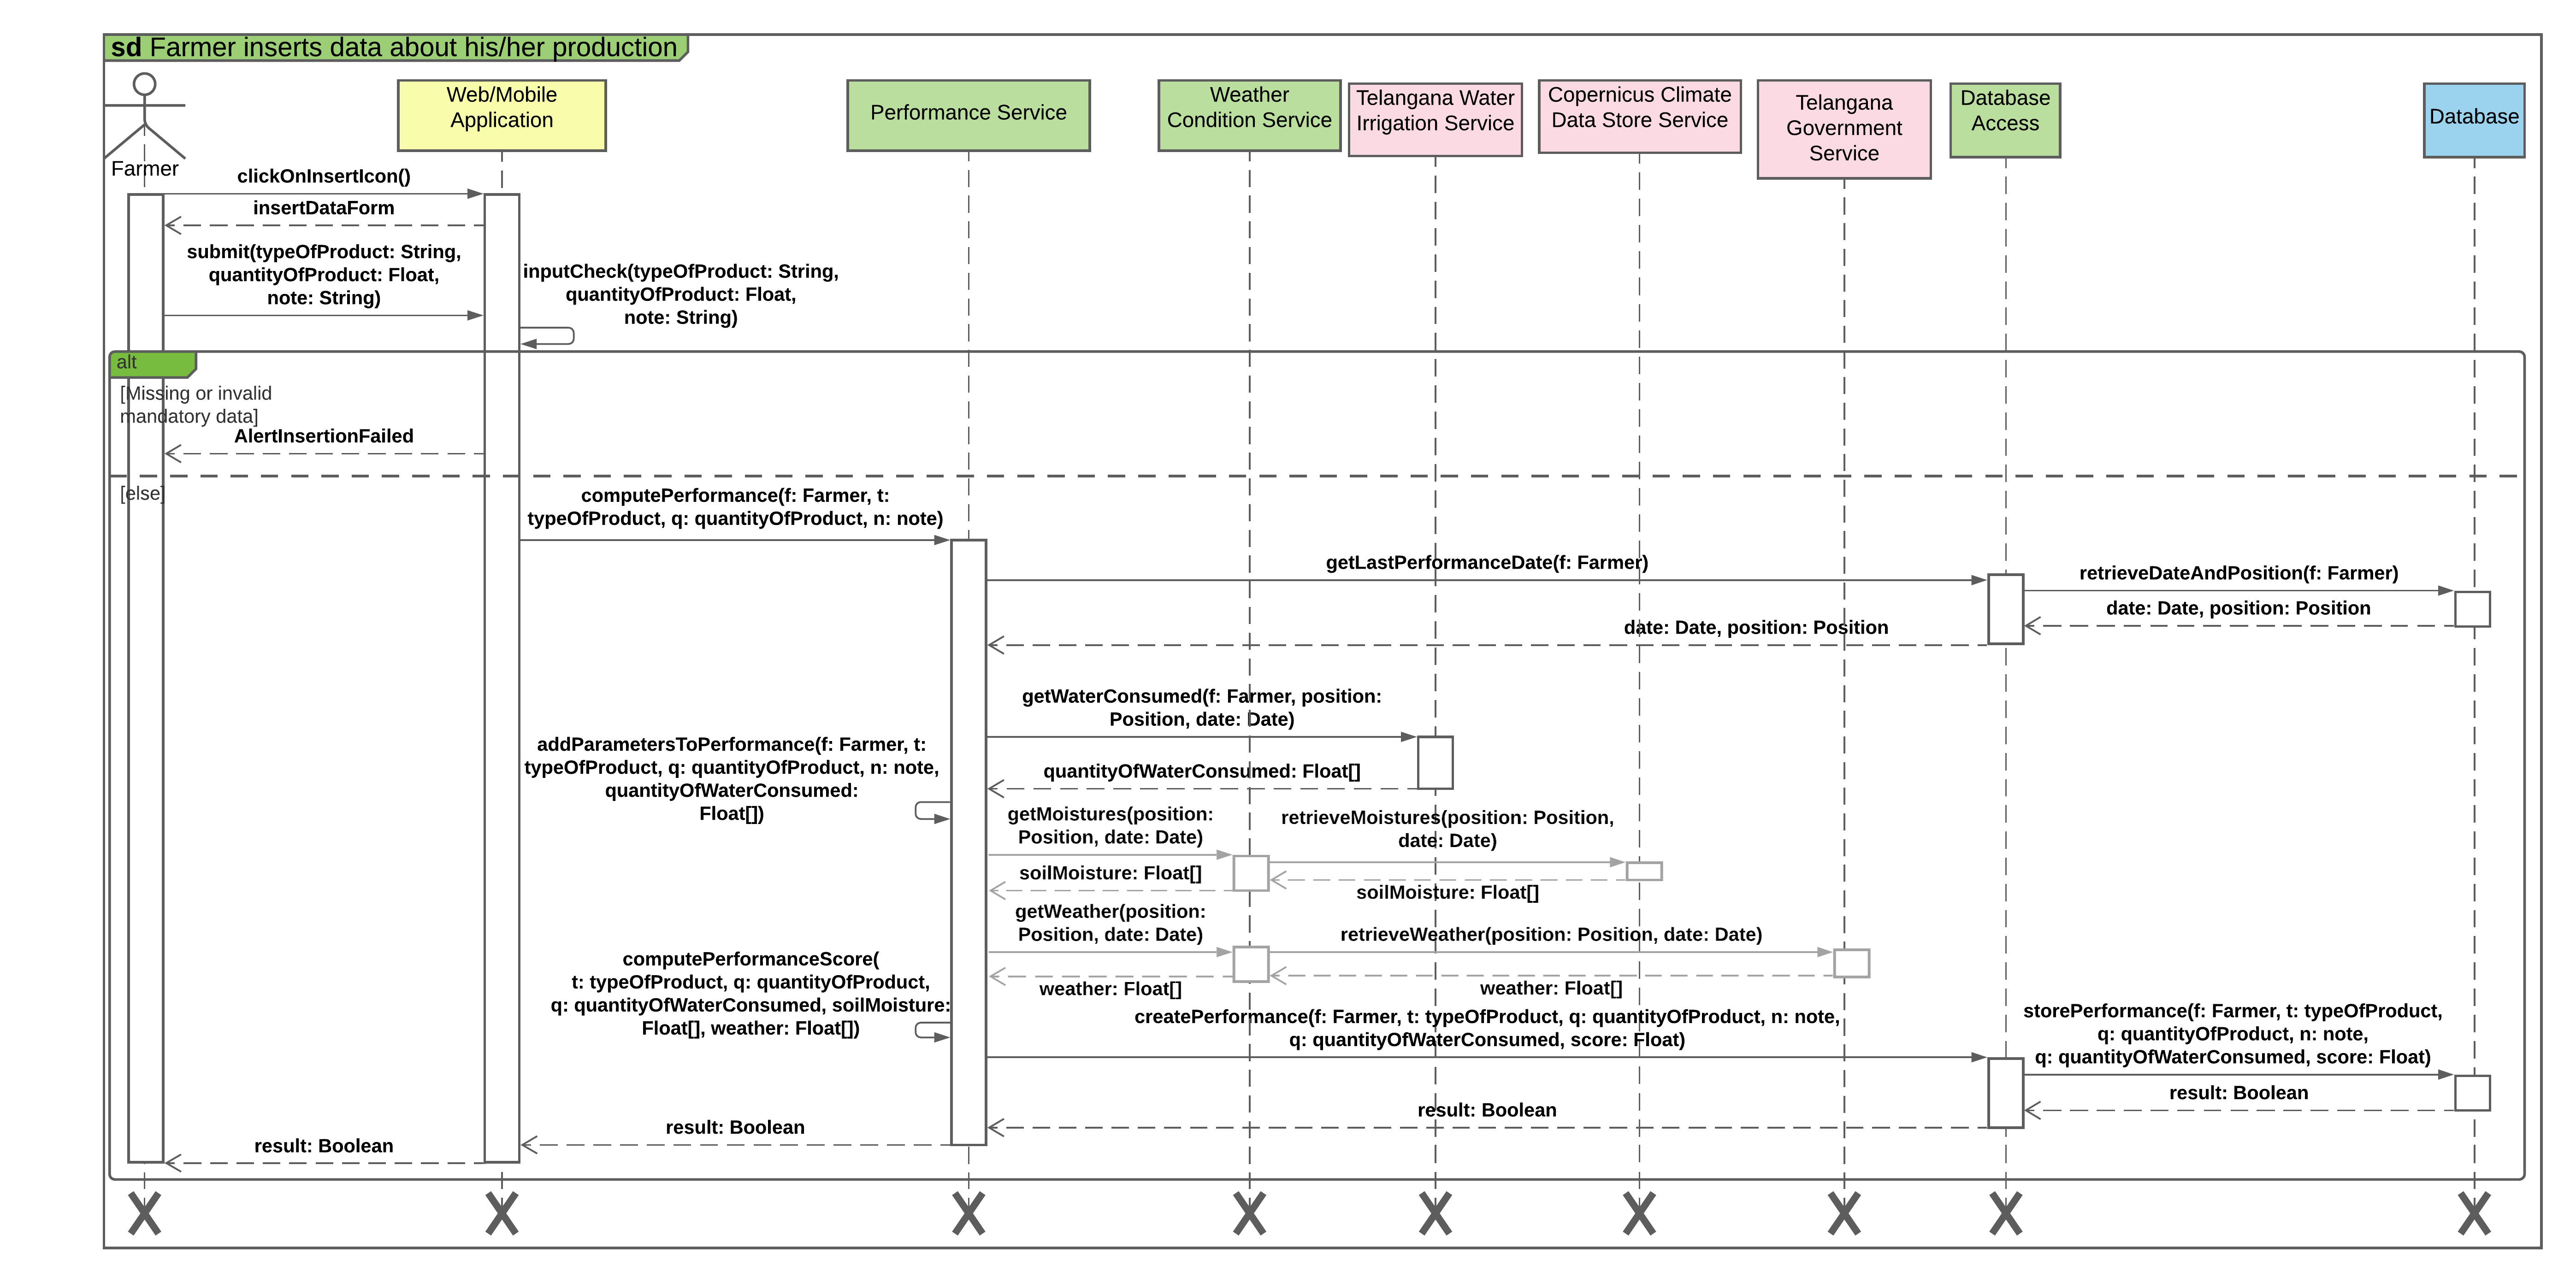
\includegraphics[scale= 0.108]{./Images/Sequence diagram/Farmer inserts data about his_her production.png}}
    \caption{Farmer inserts data about his/her production}
    \vspace*{-12cm}
\end{figure}
\fillandplacepagenumber
\end{landscape}

\subsection{DREAM sends suggestions to farmer}

This sequence diagram shows the procedure of DREAM sending periodic suggestions to a farmer who is already registered. Suggestions are computed by the system and affected by weather conditions regarding farmer's position and his/her last performance.\\
A request to compute suggestion is called by Web/MobileApplication and propagated to SuggestionService component which calls a function to get data needed to make the computation. For this reason the request is propagated through DatabaseAccess to Database. Farmer's last performance and position are eventually returned to SuggestionService. The latter component propagates two requests to get weather and soil moisture to WeatherConditionService, which is in charge to retrieve those data from external APIs (TelanganaGovernmentService and CopernicusClimateDataStoreService). Data are returned to SuggestionService which is now able to compute the suggestion calling a proper function. \\
Eventually, the suggestion is stored in the Database and is returned following the same path to Web/Mobile Application, which is able to send a notification to the farmer.

\newpage
\begin{landscape}
\begin{figure}[t!]
\vspace*{2cm}
\noindent
\centering
\centerline{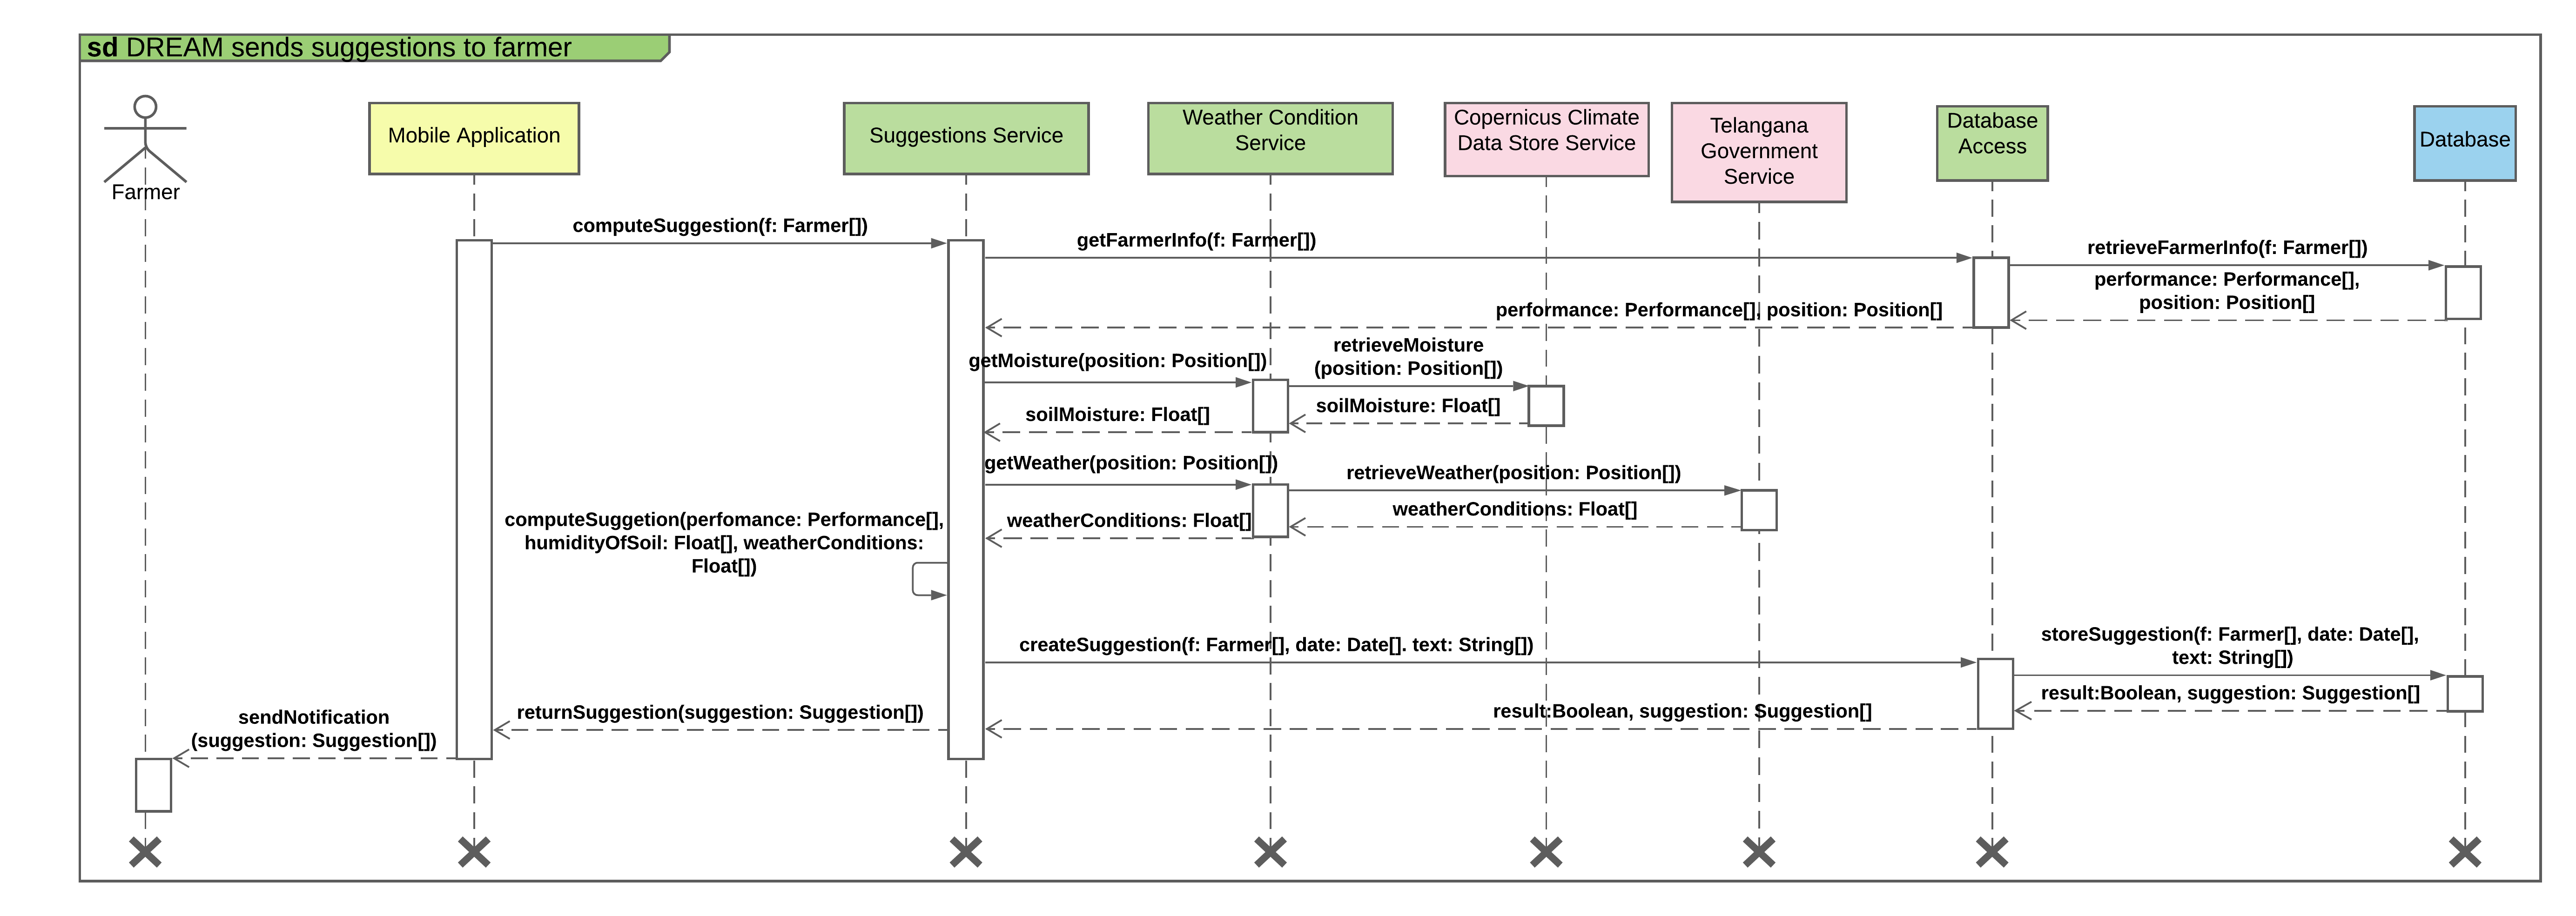
\includegraphics[scale= 0.108]{./Images/Sequence diagram/DREAM sends suggestions to farmer.png}}
    \caption{DREAM sends suggestions to farmer}
    \vspace*{-12cm}
\end{figure}
\fillandplacepagenumber
\end{landscape}

\subsection{Farmer searches for a thread in the discussion forum}

This sequence diagram shows the procedure of a farmer, already registered and logged in, searching for a thread on the discussion forum.\\
He/she clicks on \textit{discussion forum} icon. To return to the farmer the related page, Web/MobileApplication propagates a request to get all discussion forum's threads and related posts to DiscussionForumService which is able to retrieve them from the Database through DatabaseAccess.\\ 
Once the \textit{discussion forum} page is shown to the farmer, he/she clicks on \textit{search} icon and a form is returned by Web/MobileApplication. The farmer inserts the topic in the appropriated field and Web/MobileApplication calls a function to get all threads related to that topic. The request is propagated to DiscussionForumService which is in charge of finding those threads and their related posts. The result and found threads with related posts are returned to Web/MobileApplication following the same path. If result is false no thread was found and a message is sent to the user. If the result is true all found threads with related posts are shown to the farmer.

\newpage
\begin{landscape}
\begin{figure}[t!]
\vspace*{1.5cm}
\noindent
\centering
\centerline{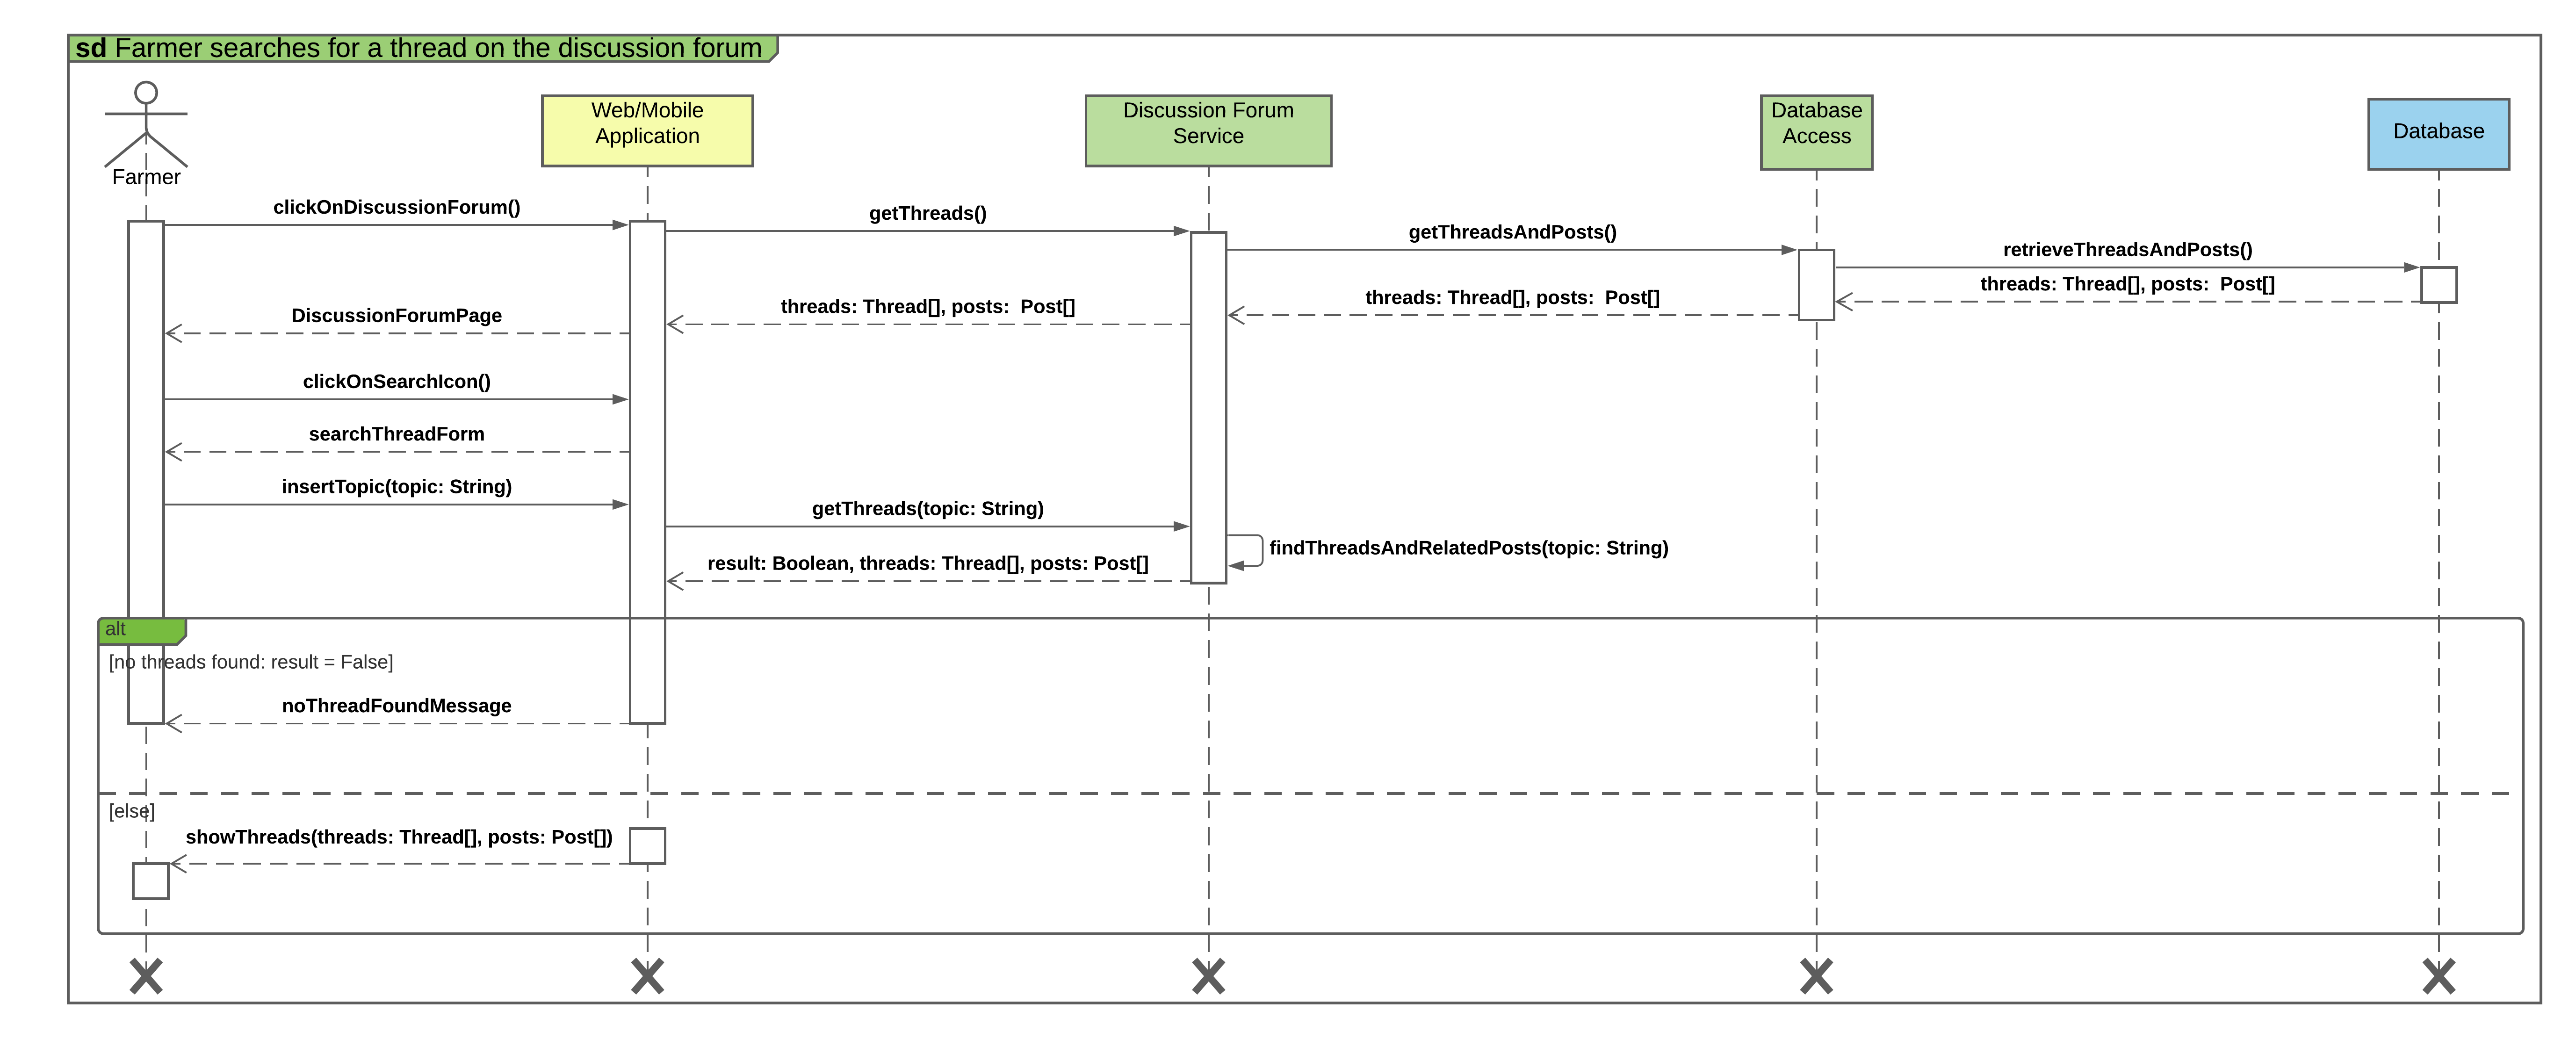
\includegraphics[scale= 0.108]{./Images/Sequence diagram/Farmer searches for a thread on the discussion forum.png}}
    \caption{Farmer searches for a thread in the discussion forum}
    \vspace*{-12cm}
\end{figure}
\fillandplacepagenumber
\end{landscape}

\subsection{Farmer creates a new thread in the discussion forum}

This sequence diagram shows the procedure of a farmer, already registered and logged in, opening a thread on the discussion forum.\\
He/she clicks on \textit{discussion forum} icon. To return to the farmer the related page, Web/MobileApplication propagates a request to get all discussion forum's threads and related posts to DiscussionForumService which is able to retrieve them from the Database through DatabaseAccess. 
Once the \textit{discussion forum} page is shown to the farmer, he/she clicks on \textit{new thread} button and a form is returned by Web/MobileApplication. The farmer inserts the topic and the text in the appropriated fields and Web/MobileApplication calls a function to store the new thread. The request is propagated to DiscussionForumService which is in charge of  adding additional information to the thread before propagating the request to Database through DatabaseAccess. The result is returned to Web/MobileApplication following the same path. If result is false the operation must be repeated.

\newpage
\begin{landscape}
\begin{figure}[t!]
\vspace*{2cm}
\noindent
\centering
\centerline{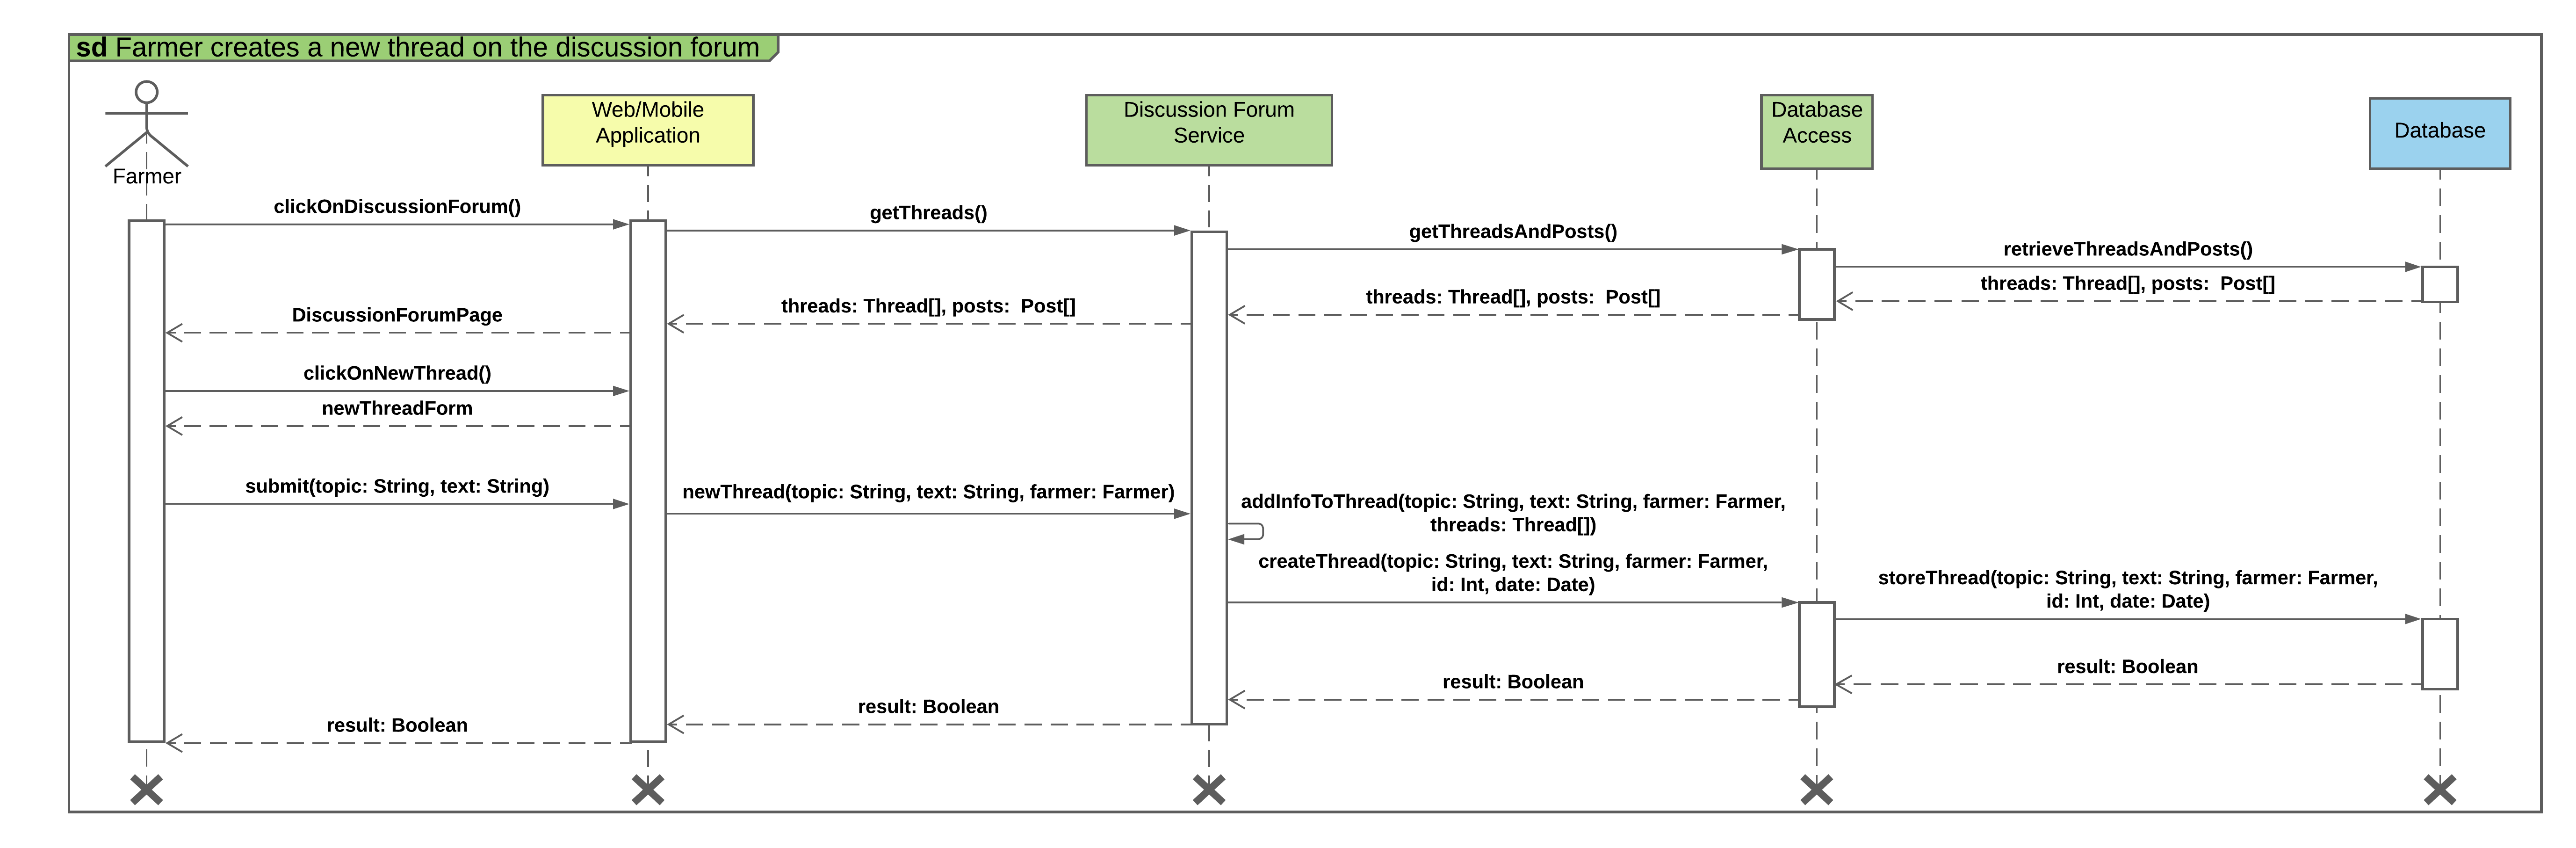
\includegraphics[scale= 0.108]{./Images/Sequence diagram/Farmer creates a new thread on the discussion forum.png}}
    \caption{Farmer creates a new thread in the discussion forum}
    \vspace*{-12cm}
\end{figure}
\fillandplacepagenumber
\end{landscape}

\subsection{Farmer replies in the discussion forum}

This sequence diagram shows the procedure of a farmer, already registered and logged in, replying on the discussion forum.\\
He/she clicks on \textit{discussion forum} icon. To return to the farmer the related page, Web/MobileApplication propagates a request to get all discussion forum's threads and related posts to DiscussionForumService which is able to retrieve them from the Database through DatabaseAccess. 
Once the \textit{discussion forum} page is shown to the farmer, he/she clicks on a thread whose details are returned by Web/MobileApplication after a function to find related posts is called. The farmer clicks on \textit{comment} button and a form is returned. He/she inserts the text of the post and Web/MobileApplication calls a function to store the new post. The request is propagated to DiscussionForumService which is in charge of  adding additional information to the post before propagating the request to Database through DatabaseAccess. The result is returned to Web/MobileApplication following the same path. If result is false the operation must be repeated. If the result is true the process is successfully completed and a message is sent to the farmer who created the post while a notification is sent to the one that has created the related thread. 

\newpage
\begin{landscape}
\begin{figure}[h]
\vspace*{-2cm}
\noindent
\centering
\centerline{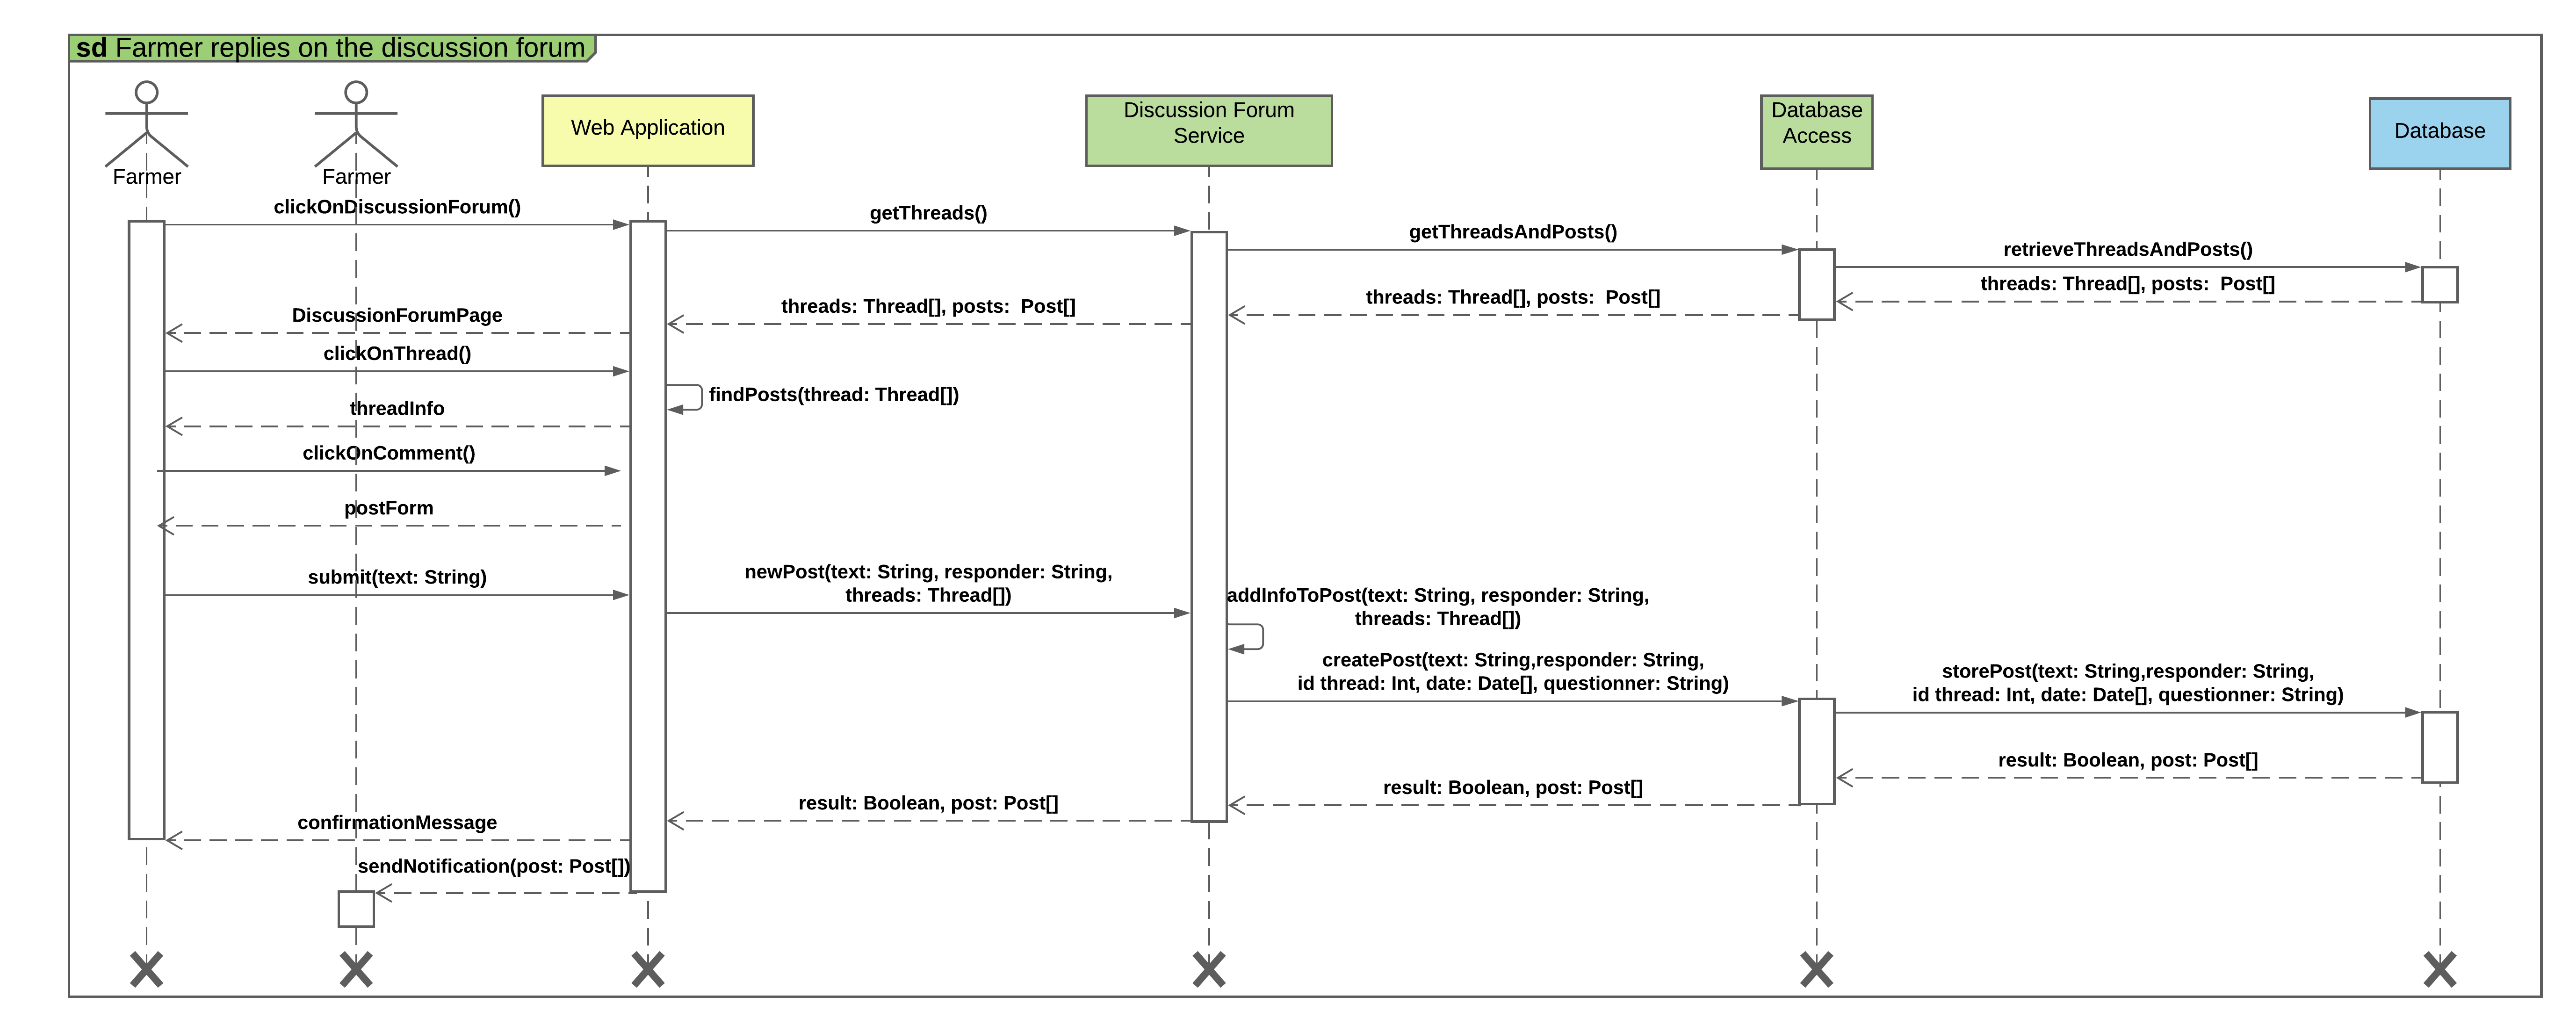
\includegraphics[scale= 0.108]{./Images/Sequence diagram/Farmer replies on the discussion forum.png}}
    \caption{Farmer replies on the discussion forum}
    \vspace*{-12cm}
\end{figure}
\fillandplacepagenumber
\end{landscape}

\subsection{Farmer creates a help request}

This sequence diagram shows the procedure of a farmer, already registered and logged in, creating a help request.\\
He/she clicks on \textit{help request} icon. To return to the farmer the related page, Web/MobileApplication propagates a request to get all help requests and related help responses related to the farmer to HelpRequestService which is able to retrieve them from the Database through DatabaseAccess. 
Once the \textit{help request} page is shown to the farmer, he/she clicks on \textit{create help request} button and a form is returned by Web/MobileApplication. The farmer inserts the text in the appropriated field and checks well performing farmers as recipient if he/she wants to. Web/MobileApplication calls a function to store the new help request. The request is propagated to HelpRequestService which is in charge of  adding additional information to the help request before returning it following the same path to show its details to the farmer. The help request is then stored in the Database. The result and the help request are returned to Web/MobileApplication following the same path. If result is false the operation must be repeated. If it is true a notification is always sent to the agronomist responsible of the mandal which the farmer is located in. If well performing farmers are also checked as recipient a function is called by PerformanceService to get well performing farmers given all farmers' performances. The farmers retrieved are returned to Web/MobileApplication which is now able to send them a notification about the new help request received. 

\newpage
\begin{landscape}
\begin{figure}[h]
\vspace*{-2cm}
\noindent
\centering
\centerline{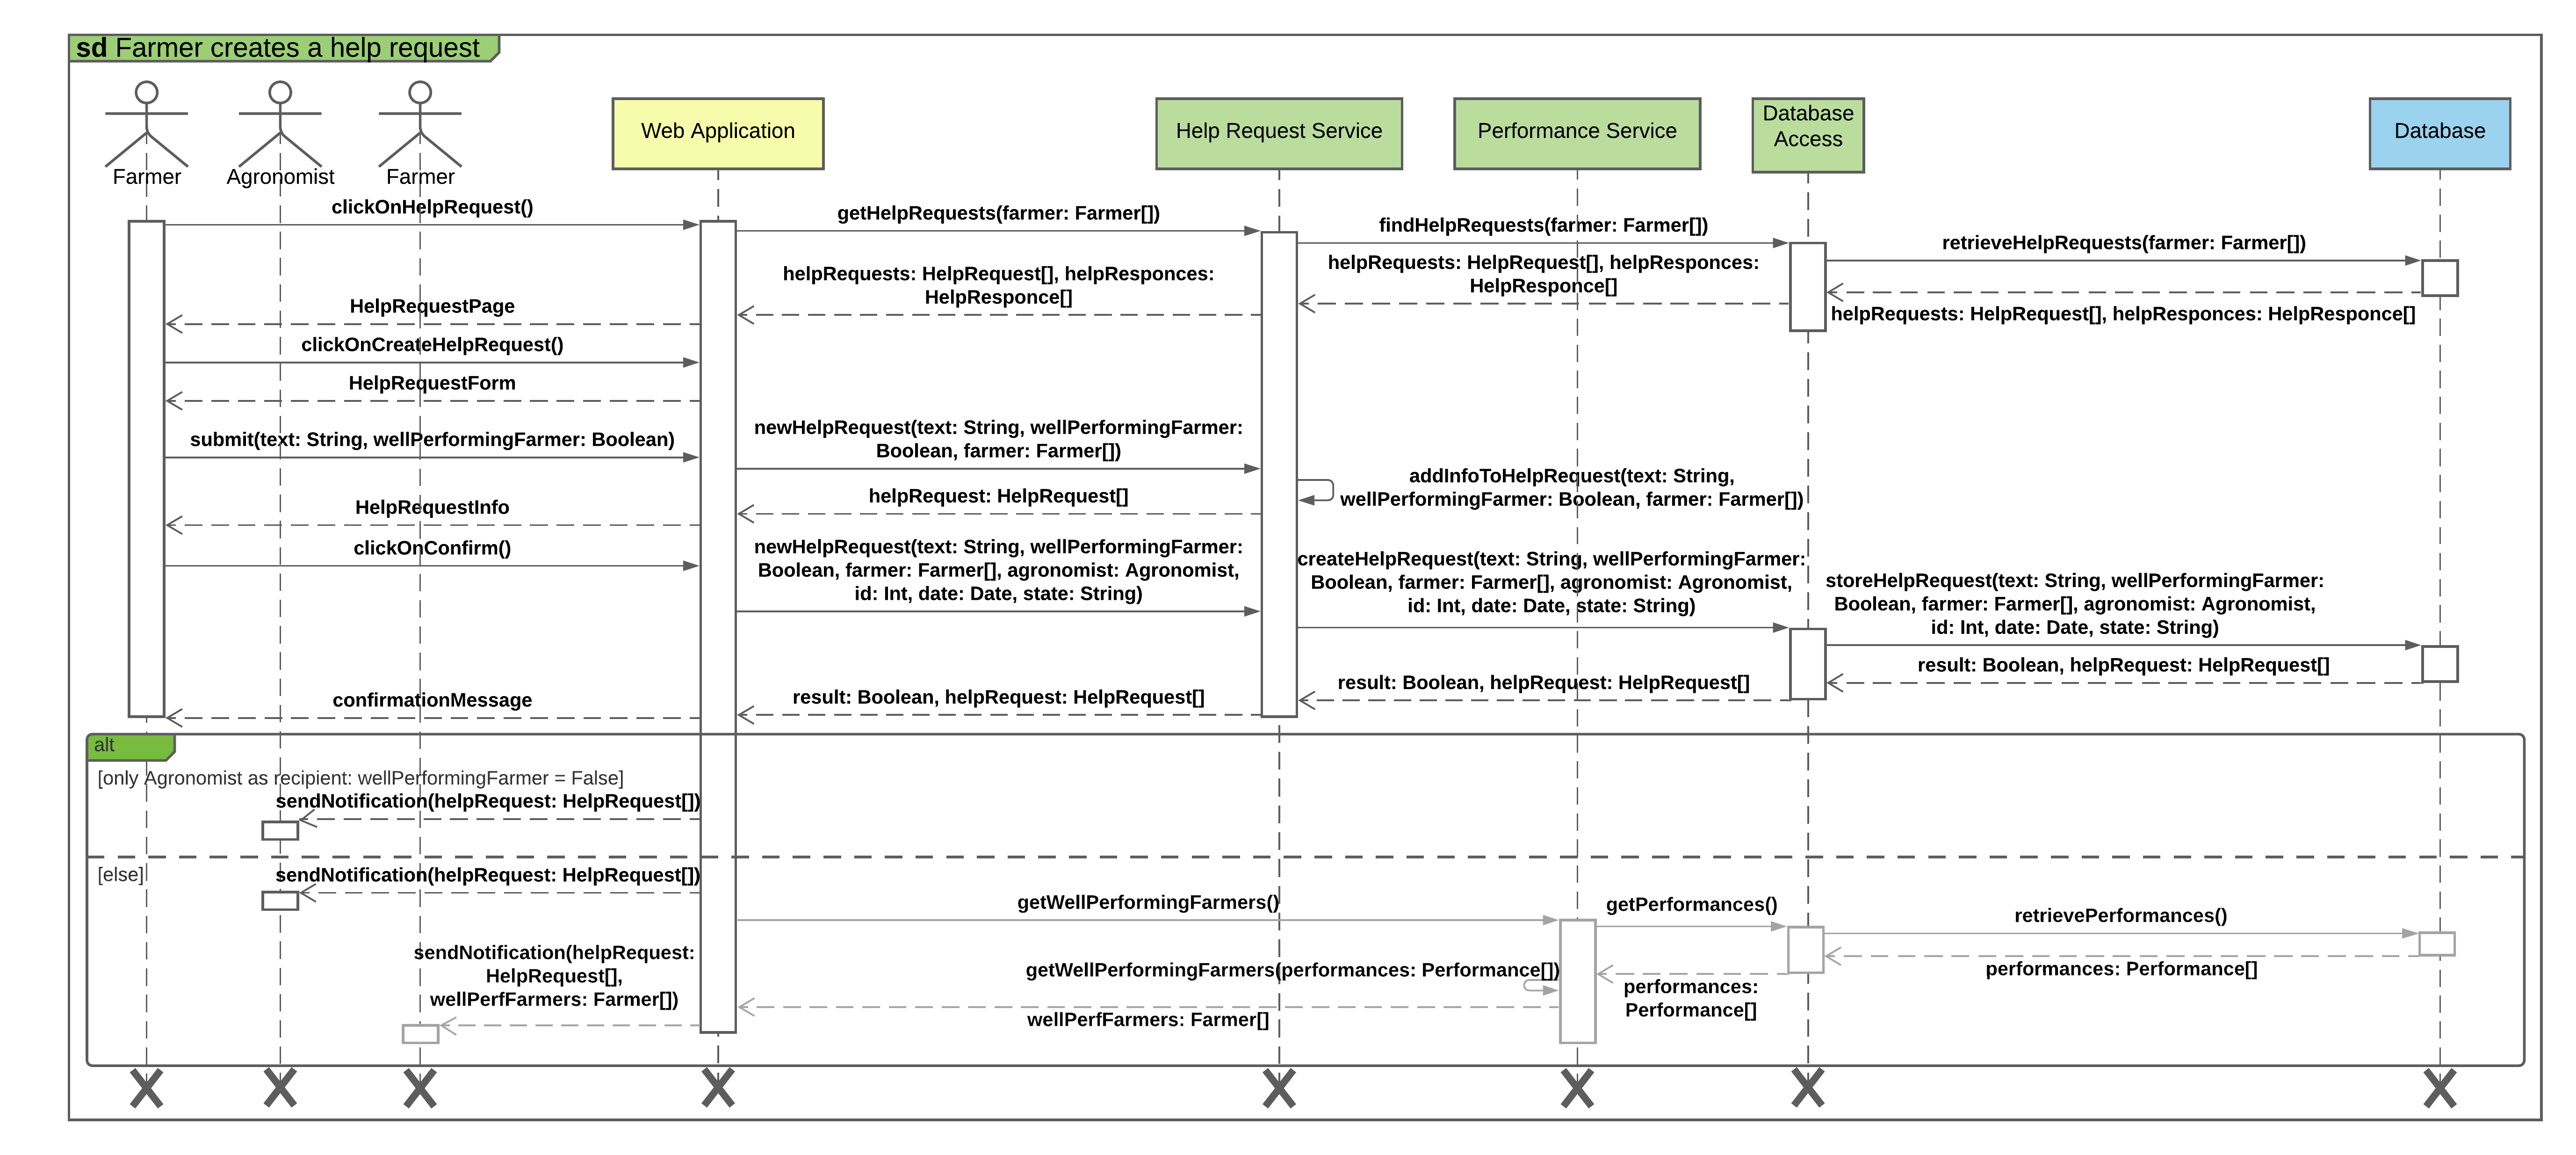
\includegraphics[scale= 0.108]{./Images/Sequence diagram/Farmer creates a help request.png}}
    \caption{Farmer creates a help request}
    \vspace*{-12cm}
\end{figure}
\fillandplacepagenumber
\end{landscape}

\subsection{Agronomist replies to a help request}

This sequence diagram shows the procedure of an agronomist, already registered and logged in, replying to a help request. The same functionality can be performed by a well performing farmer if he/she is checked as recipient in the help request.\\
The agronomist clicks on \textit{help request} icon. To return to the agronomist the related page, Web/MobileApplication propagates a request to get all help requests related to the agronomist to HelpResponseService which is able to retrieve them from the Database through DatabaseAccess. 
Once the \textit{help request} page is shown to the agronomist, he/she clicks on \textit{reply} button and a form is returned by Web/MobileApplication. The agronomist inserts the text in the appropriated field and Web/MobileApplication calls a function to store the new help response. The request is propagated to HelpResponseService which is in charge of  adding additional information to the help response. The help response is then stored in the Database. The result and the help response are returned to Web/MobileApplication following the same path. If result is false the operation must be repeated. If it is true a notification is sent to the farmer who made the help request and a confirmation message is sent to the agronomist.

\newpage
\begin{landscape}
\begin{figure}[t!]
\vspace*{1cm}
\noindent
\centering
\centerline{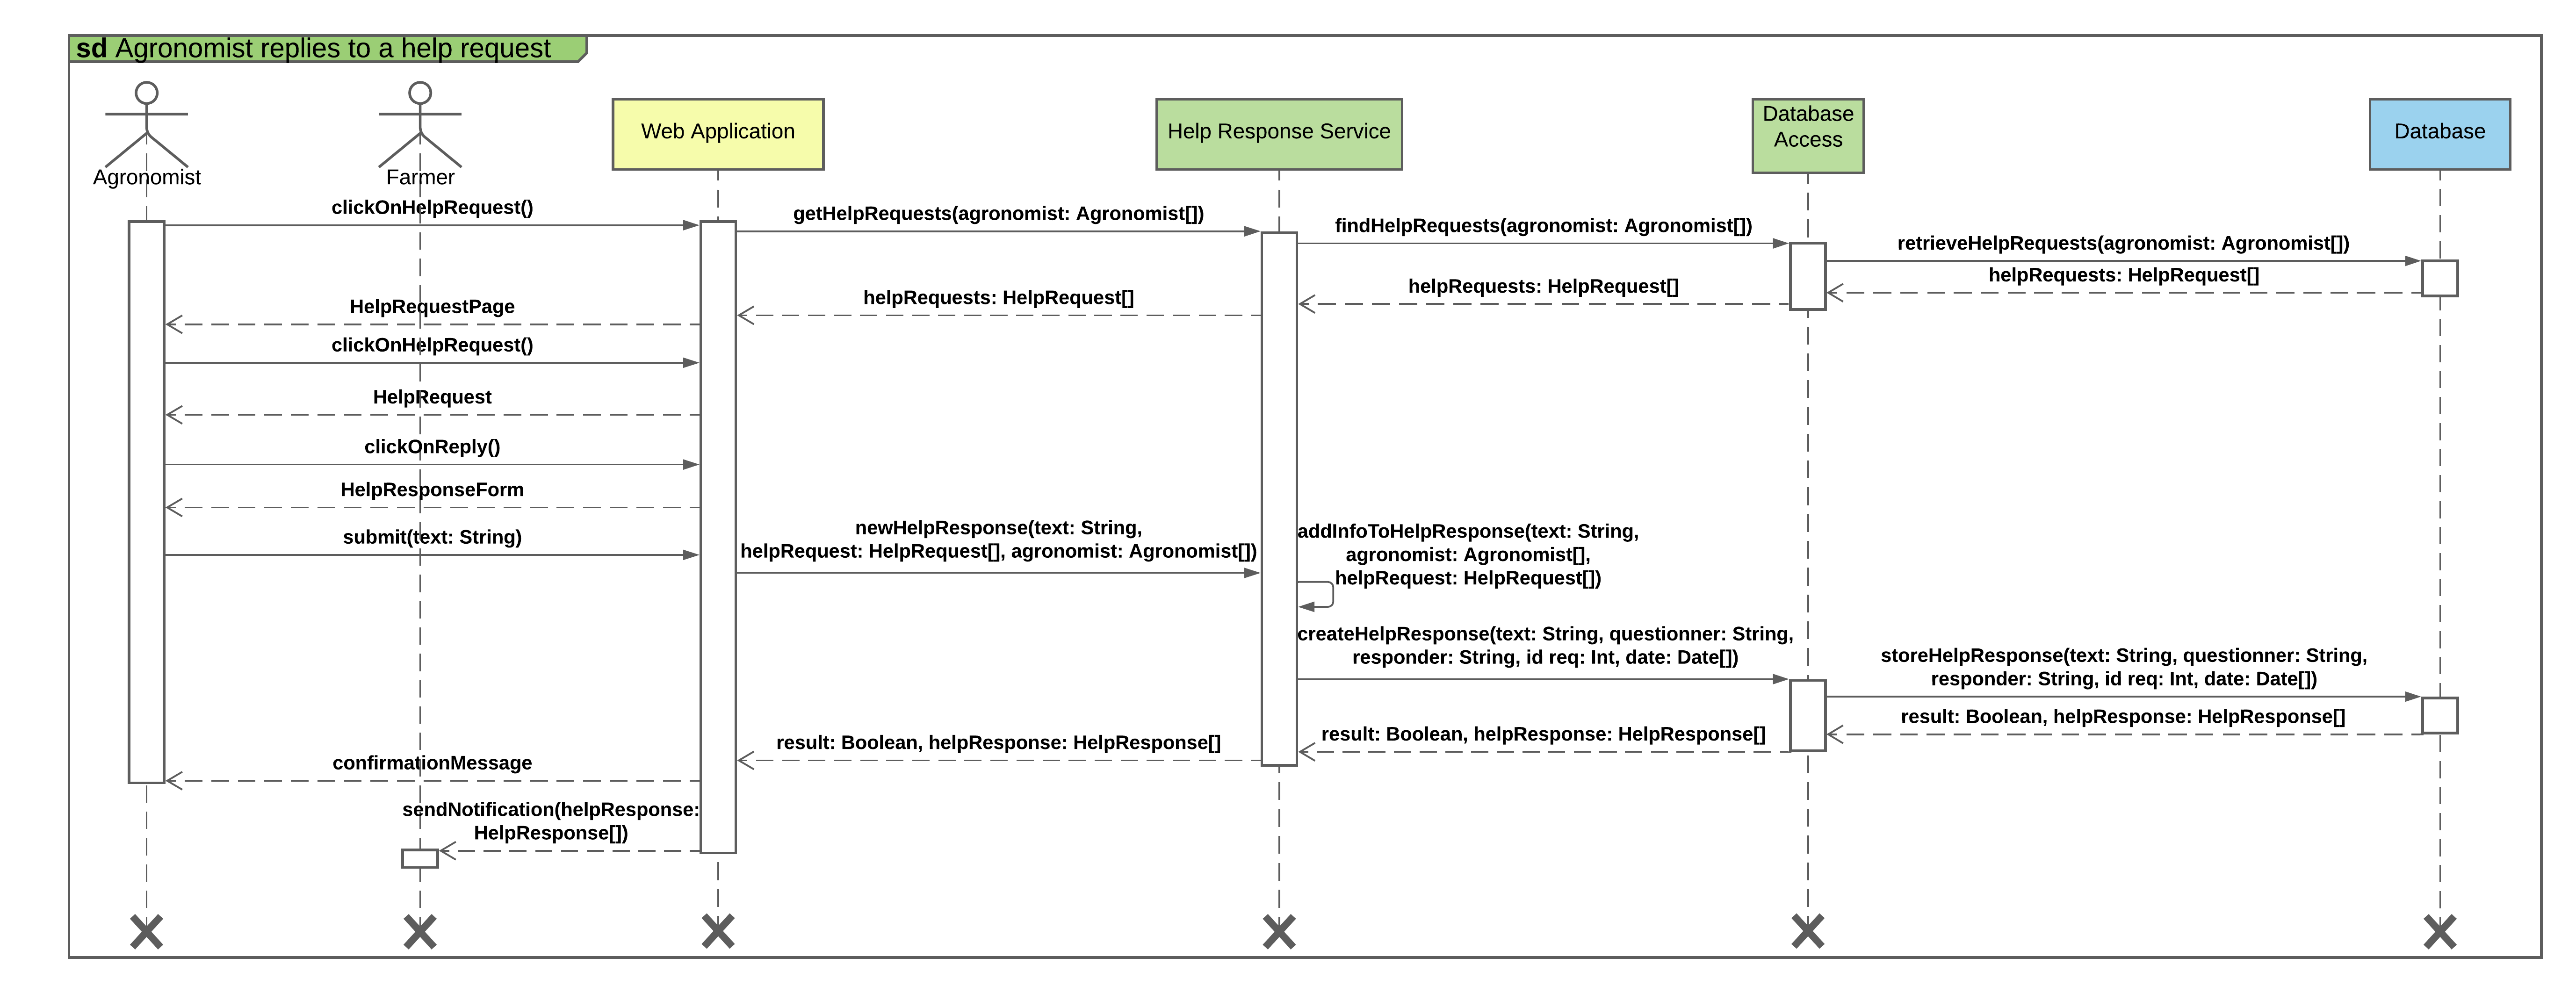
\includegraphics[scale= 0.108]{./Images/Sequence diagram/Agronomist replies to a help request.png}}
    \caption{Agronomist replies to a help request}
    \vspace*{-12cm}
\end{figure}
\fillandplacepagenumber
\end{landscape}

\subsection{Farmer solves a help request}

This sequence diagram shows the procedure of a farmer, already registered and logged in, solving a help request.\\
The farmer clicks on \textit{help request} icon. To return to the farmer the related page, Web/MobileApplication propagates a request to get all help requests and help responses related to the farmer to HelpRequestService which is able to retrieve them from the Database through DatabaseAccess. 
Once the \textit{help request} page is shown to the farmer, he/she clicks on \textit{my help requests} button to visualize those created by him/her and the related page is returned by Web/MobileApplication. The farmer solves a help request clicking on the related button and Web/MobileApplication calls a function to update the status of the help request. The request is propagated to HelpRequestService and then the help request state is updated in the Database. The result is returned to Web/MobileApplication following the same path. If result is false the operation must be repeated.

\newpage
\begin{landscape}
\begin{figure}[t!]
\vspace*{2cm}
\noindent
\centering
\centerline{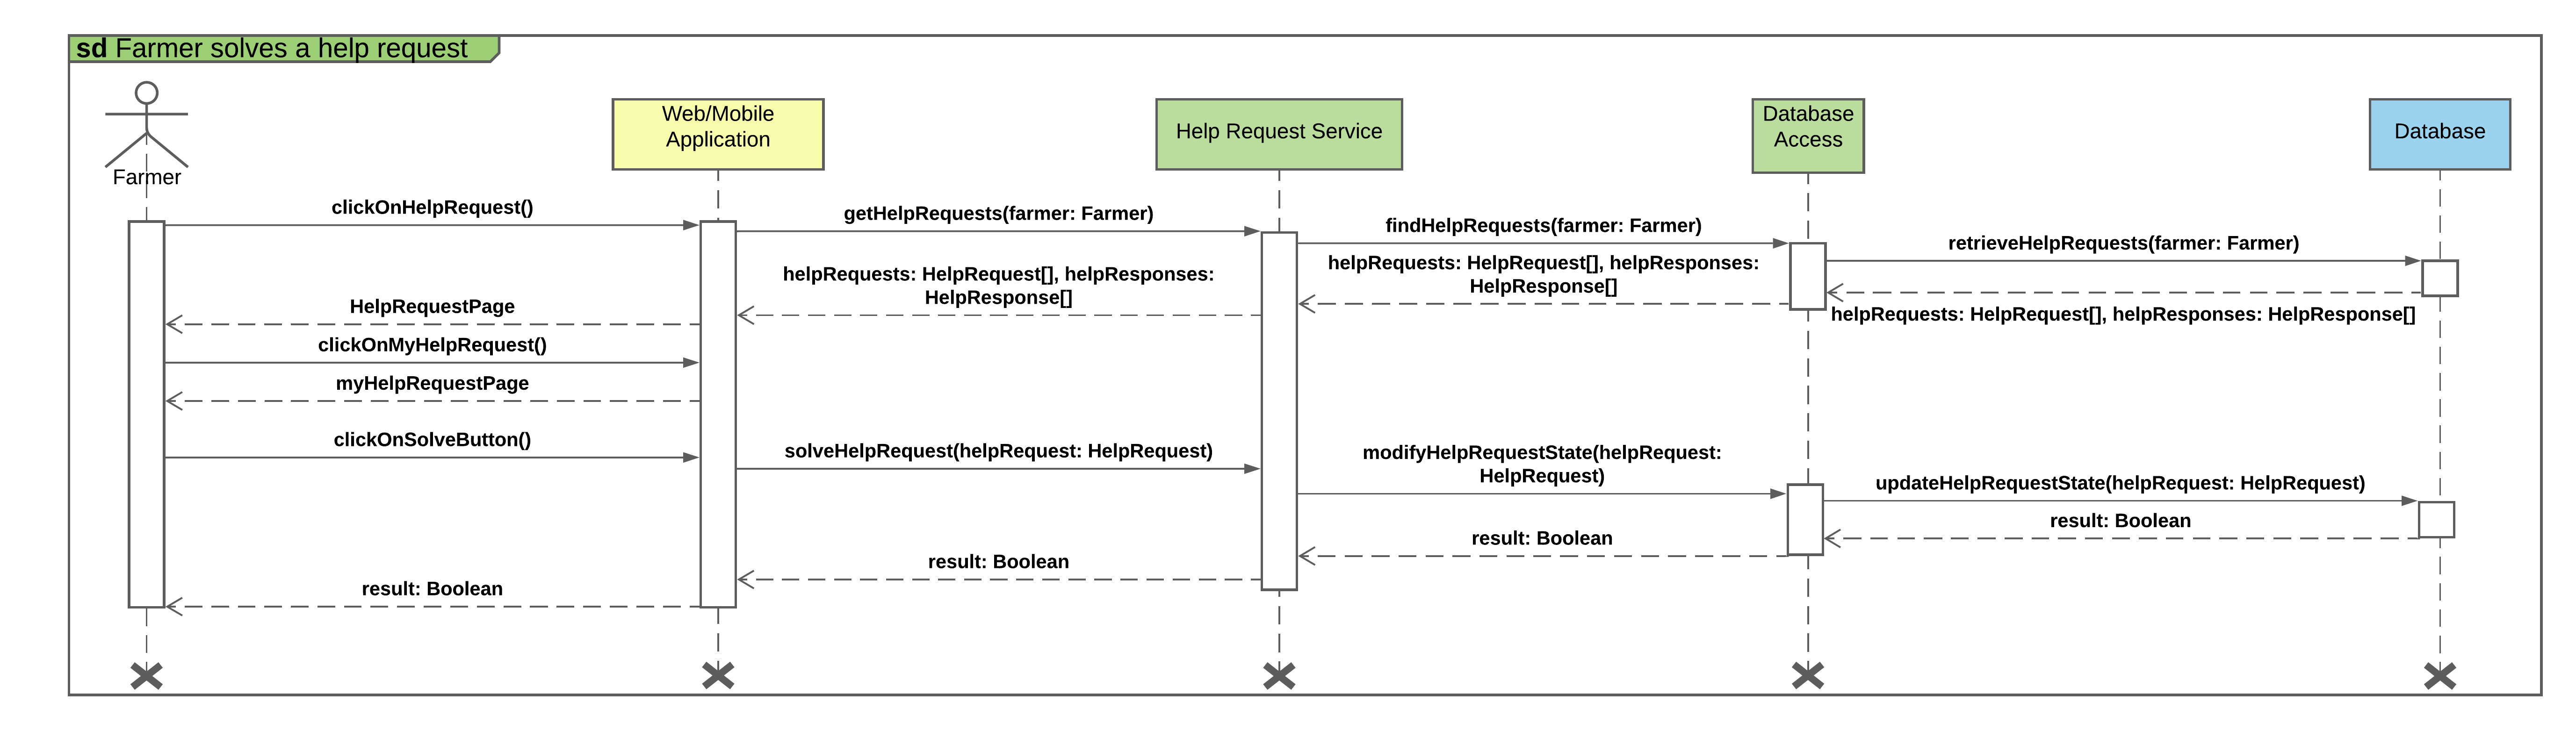
\includegraphics[scale= 0.108]{./Images/Sequence diagram/Farmer solves a help request.png}}
    \caption {Farmer solves a help request}
    \vspace*{-12cm}
\end{figure}
\fillandplacepagenumber
\end{landscape}

\subsection{Agronomist visualizes weather conditions}

This sequence diagram shows the procedure of an agronomist, already registered and logged in, visualizing weather conditions.\\
The agronomist clicks on \textit{weather} icon.
He/she can optionally select the date (from the current day up to seven days) for which he/she wants to visualize data. By default, if he/she doesn't select anything, the system shows him/her weather conditions for the current day. To return to the agronomist the related page, Web/MobileApplication propagates a request to get the weather map of his/her mandal to WeatherForecastsService which is able to retrieve weather and soil moisture data from external APIs (TelanganaGovernmentService and CopernicusClimateDataStoreService).
Then, data retrieved are returned to WeatherForecastsService which is in charge also of processing the mandal weather map interacting with GoogleMapsAPI.  
Eventually, the map is shown to the agronomist.

\newpage
\begin{landscape}
\begin{figure}[t!]
\vspace*{1.5cm}
\noindent
\centering
\centerline{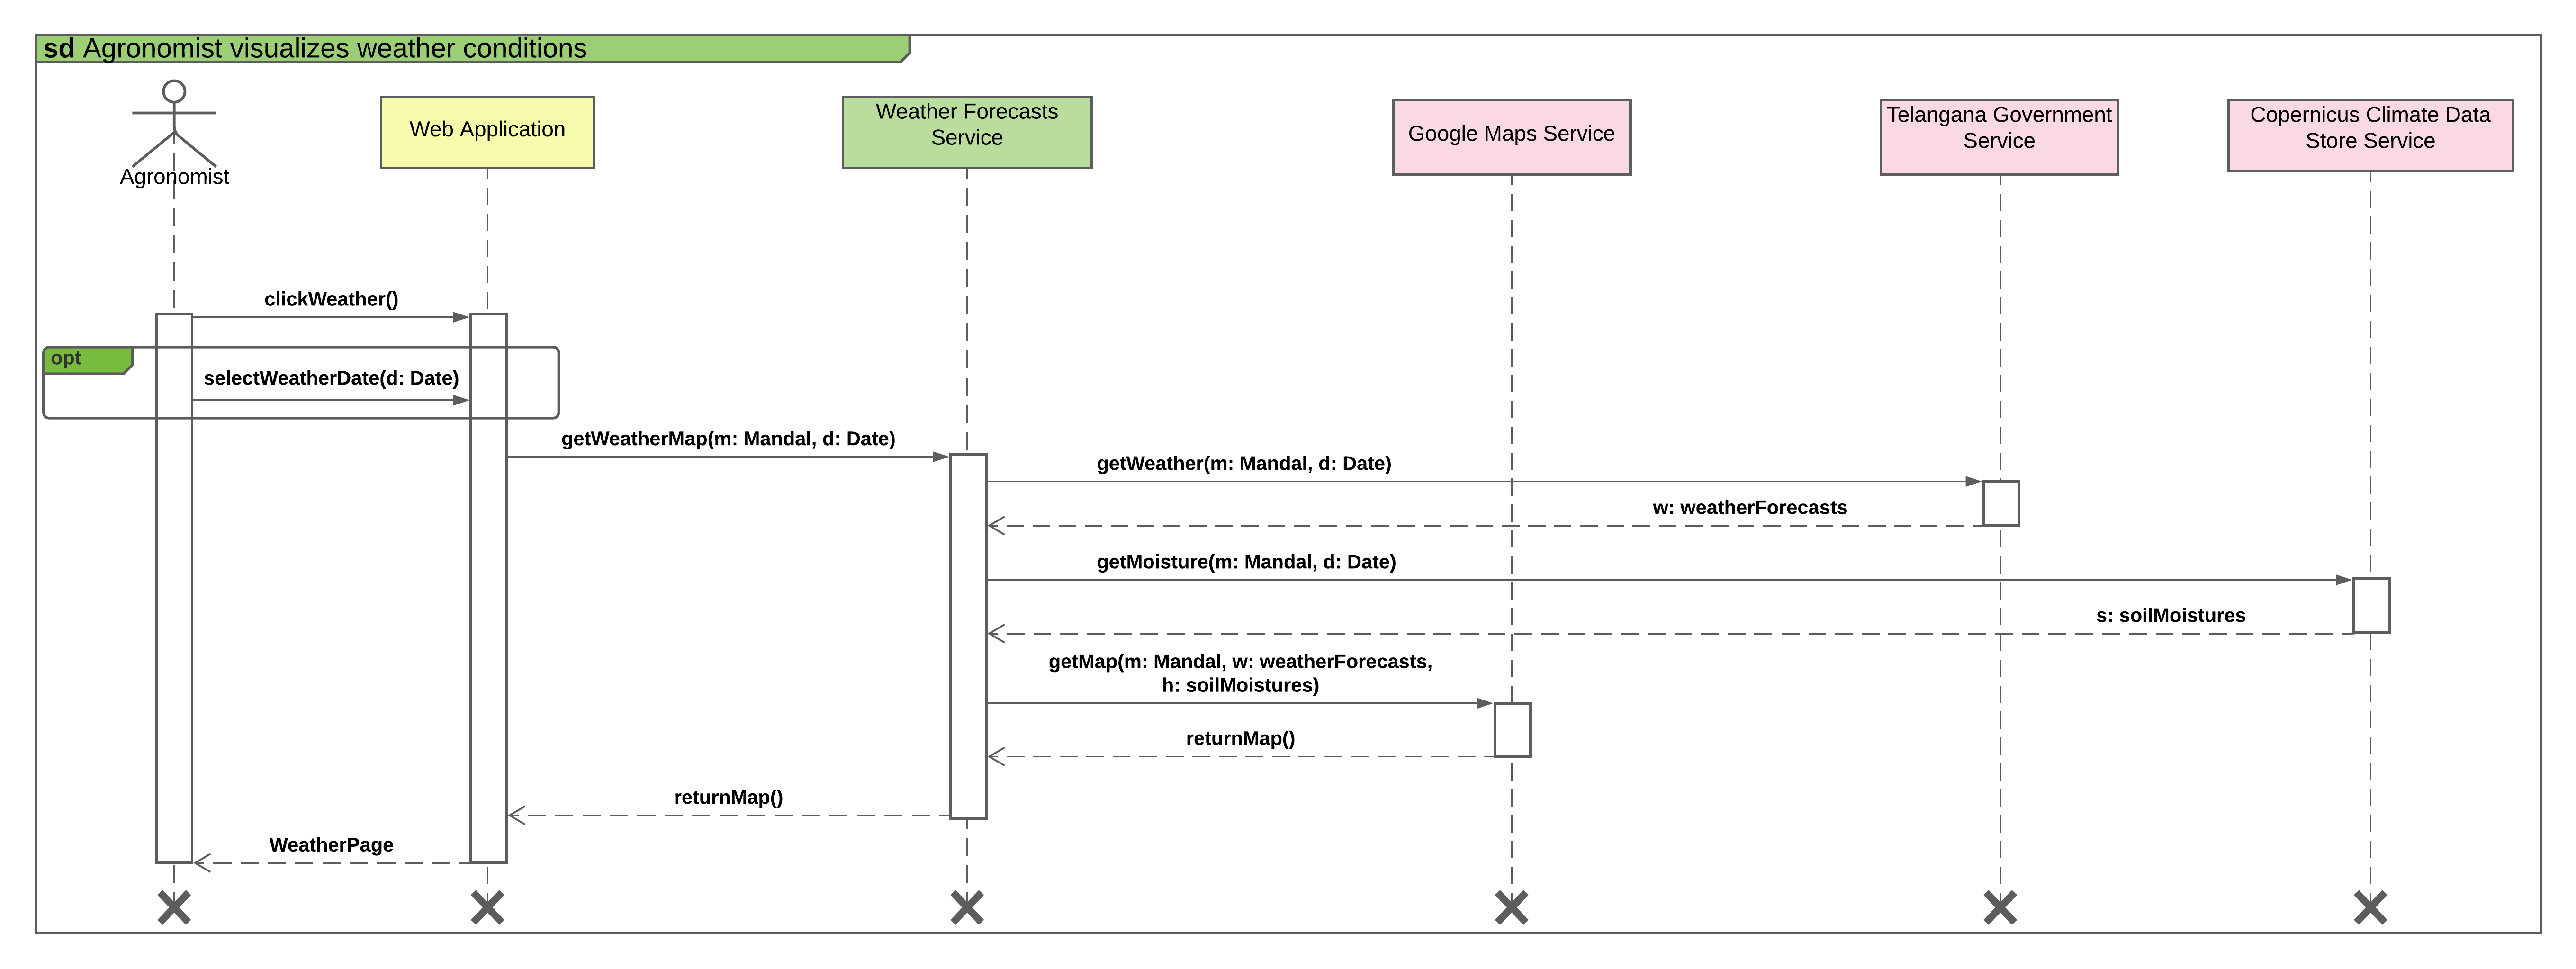
\includegraphics[scale= 0.108]{./Images/Sequence diagram/Agronomist visualizes weather conditions.png}}
    \caption{Agronomist visualizes weather conditions}
    \vspace*{-12cm}
\end{figure}
\fillandplacepagenumber
\end{landscape}

\subsection{Agronomist visualizes and analyzes farmers' data}

This sequence diagram shows the procedure of an agronomist, already registered and logged in, visualizing and analyzing his/her mandal's farmers' data in the homepage of the application.\\
The agronomist opens the application. 
Web/MobileApplication propagates two requests, one to TableService to get a table of farmers' performances in descending order and the other one to MandalMapService to get the mandal map on which are displayed farmers's performances scores. For both services it is necessary to retrieve from the Database mandal's farmers' data (including performances and positions). Those data are returned to TableService and to MandalMapService. The latter component is in charge of processing the map to be displayed to the agronomist, for this reason it interacts with GoogleMapAPI external service.
Eventually the \textit{homepage} is shown to the agronomist.

\newpage
\begin{landscape}
\begin{figure}[t!]
\vspace*{1.5cm}
\noindent
\centering
\centerline{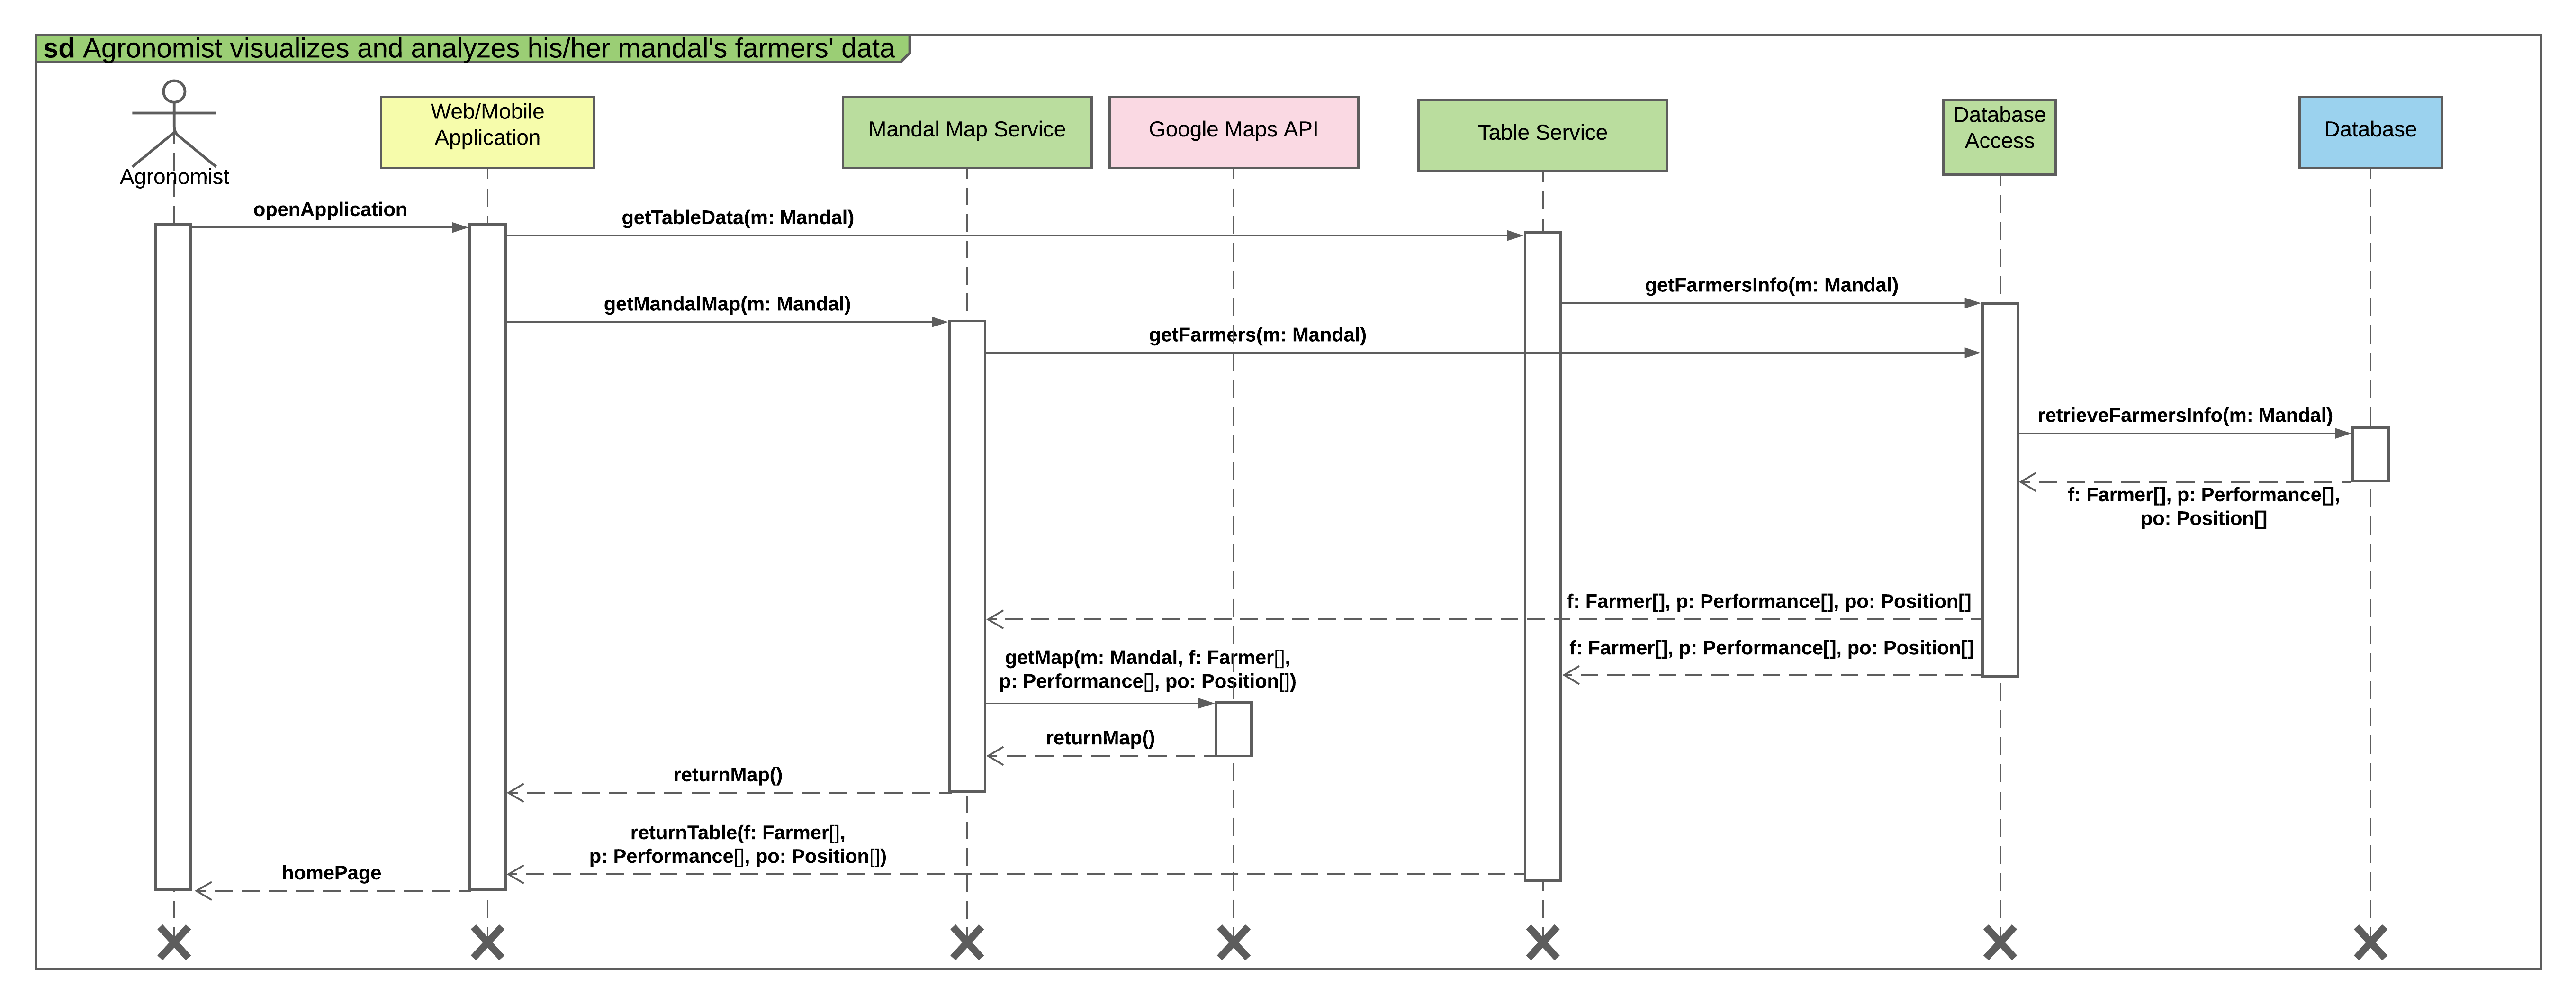
\includegraphics[scale= 0.108]{./Images/Sequence diagram/Agronomist visualizes and analyzes his_her mandal's farmers' data.png}}
    \caption{Agronomist visualizing and analyzing farmers' data}
    \vspace*{-12cm}
\end{figure}
\fillandplacepagenumber
\end{landscape}

\subsection{Agronomist updates his/her daily plan}

This sequence diagram shows the procedure of an agronomist, already registered and logged in, updating his/her daily plan.\\
The agronomist clicks on \textit{daily plan} icon. To return to the agronomist the related page, Web/MobileApplication propagates a request to get all daily plans and visits related to the agronomist to DailyPlanService which is able to retrieve them from the Database through DatabaseAccess. 
Once the \textit{daily plan} page is shown to the agronomist, he/she clicks on \textit{update} button. The update form is returned by Web/MobileApplication. The agronomist fills out the form and a function is called by Web/MobileApplication to get the visit corresponding to date and hour inserted by the agronomist. The function is propagated to DailyPlanService which is in charge of finding the visit and returns it following the same path. If result is false no visit was found and a new visit is created and stored in the Database. If result is true a visit with the date and hour inserted by the agronomist already exists, for this reason it is updated in the database according to the information entered by the user. In both cases, the visit's status is set into scheduled and the corresponding daily plan's state is change into updated. 
Eventually the result and the visit are returned following the same path and a notification is sent to the farmer whose visit has been created/changed.

\newpage
\begin{landscape}
\begin{figure}[h]
\vspace*{-2cm}
\noindent
\centering
\centerline{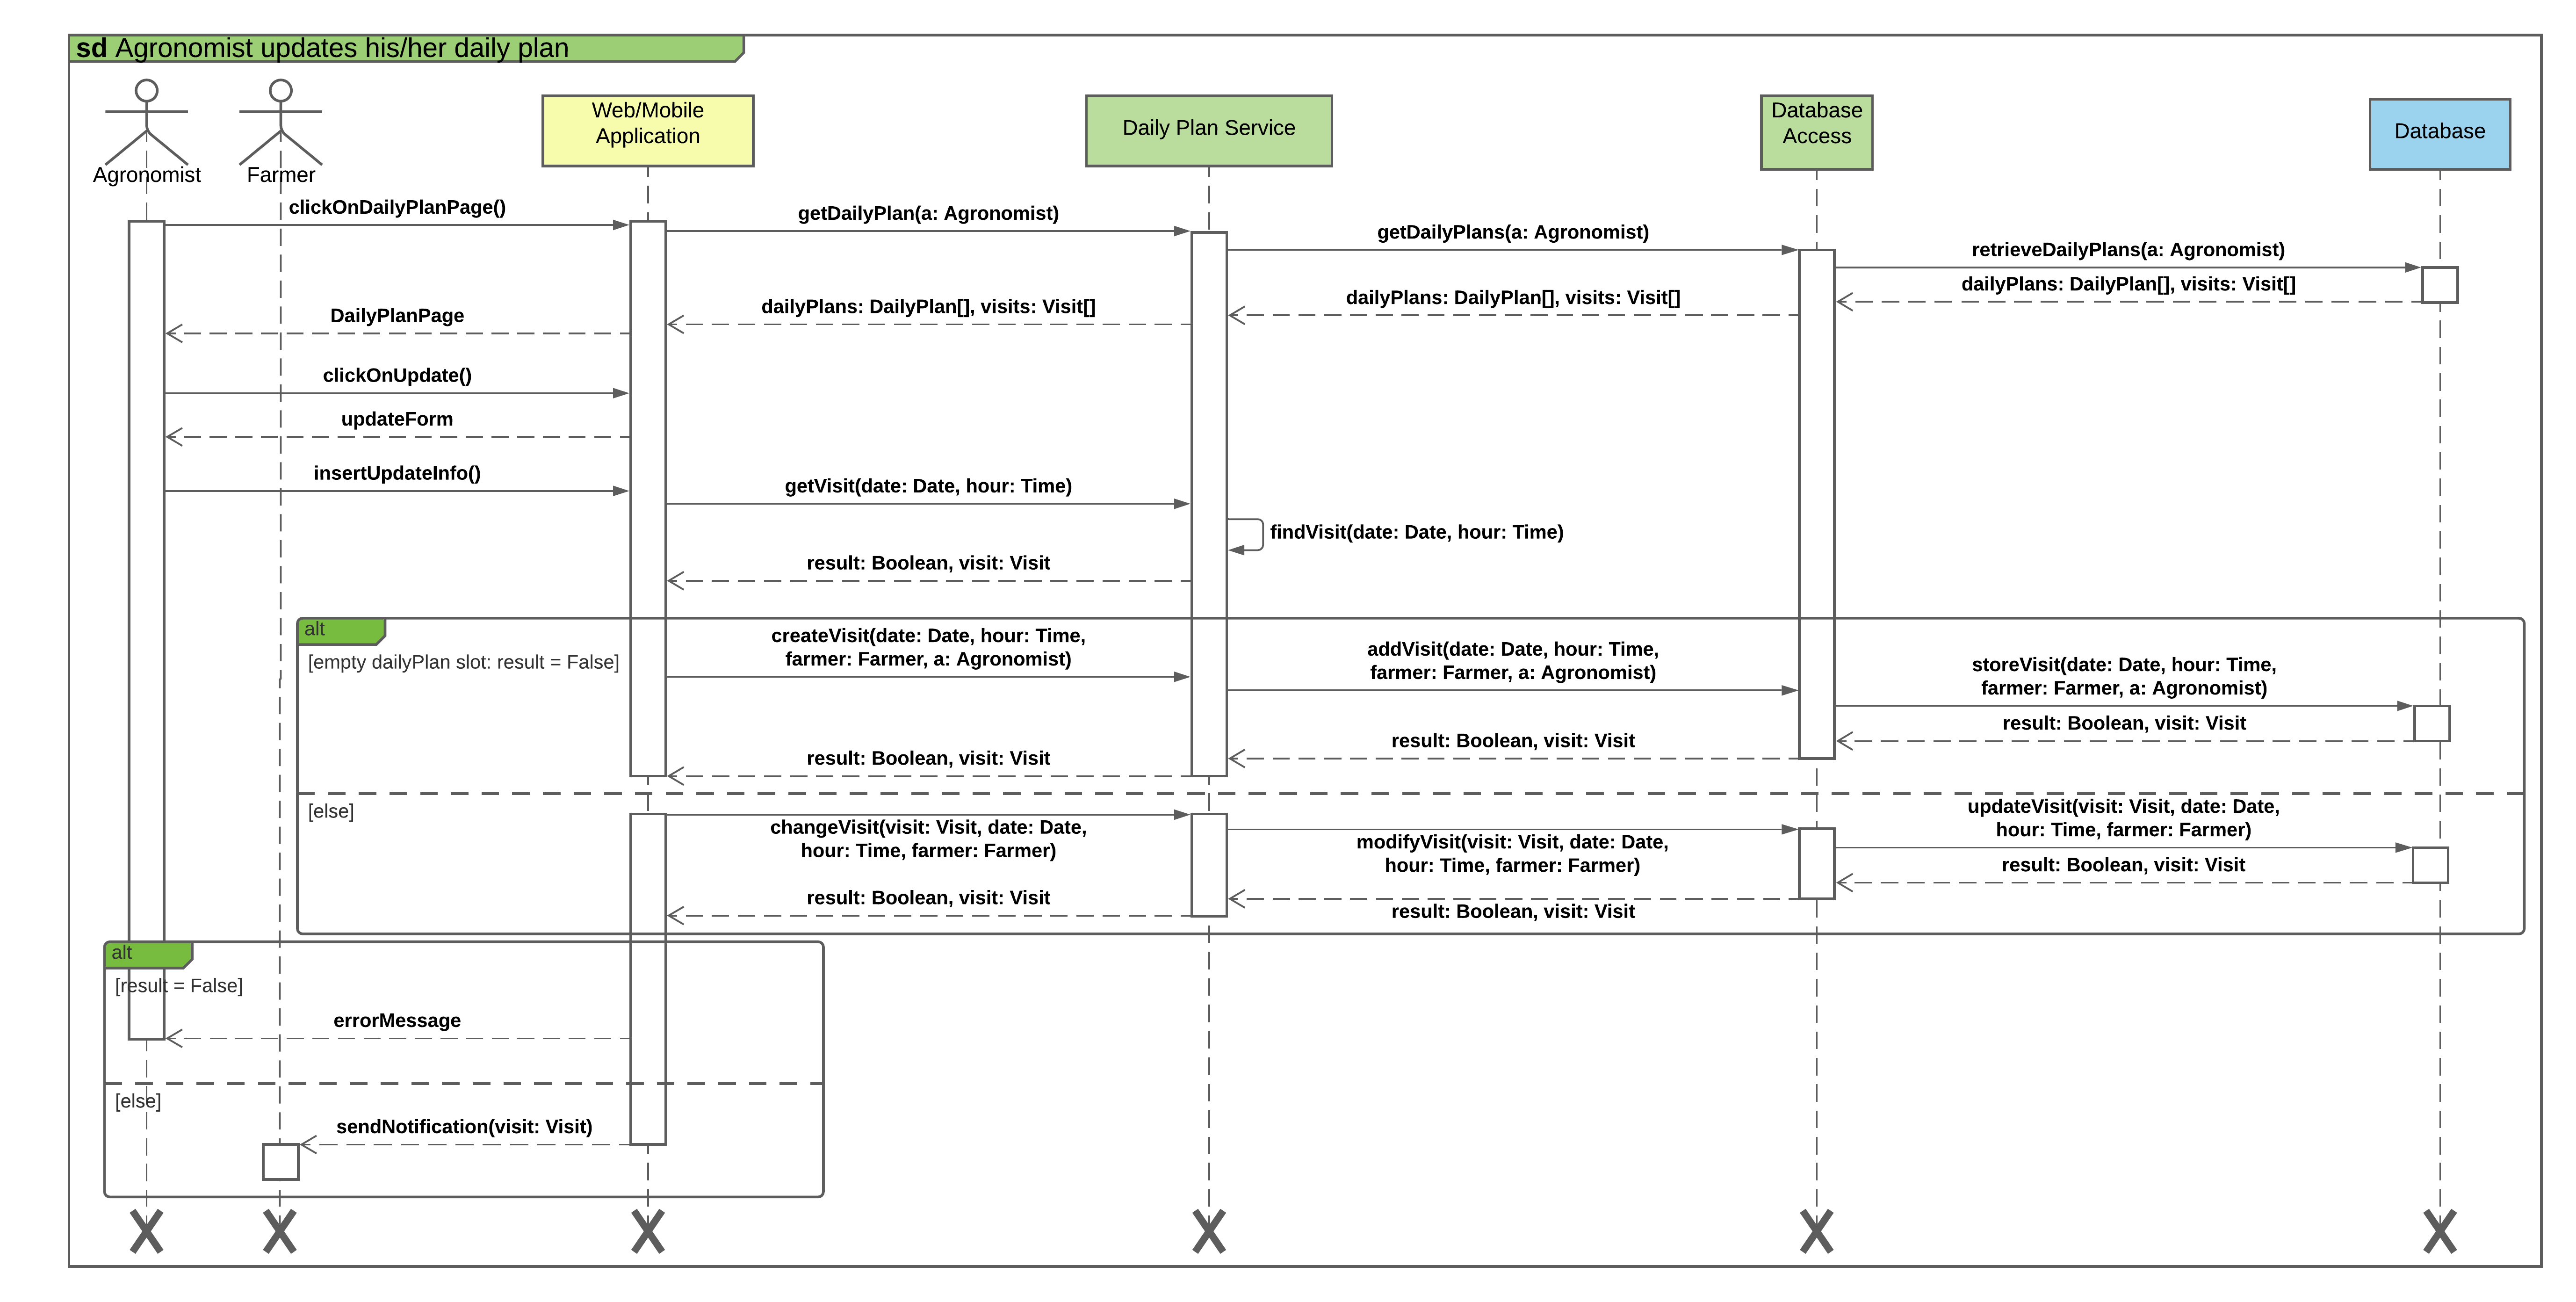
\includegraphics[scale= 0.108]{./Images/Sequence diagram/Agronomist updates his_her daily plan.png}}
    \caption{Agronomist updates his/her daily plan}
    \vspace*{-12cm}
\end{figure}
\fillandplacepagenumber
\end{landscape}


\subsection{Agronomist confirms his/her daily plan}

This sequence diagram shows the procedure of an agronomist, already registered and logged in, confirming his/her daily plan.\\
The agronomist clicks on \textit{daily plan} icon. To return to the agronomist the related page, Web/MobileApplication propagates a request to get all daily plans and visits related to the agronomist to DailyPlanService which is able to retrieve them from the Database through DatabaseAccess. 
Once the \textit{daily plan} page is shown to the agronomist, he/she clicks on a certain daily plan page and a function to retrieve the selected daily plan and related visits is called by Web/MobileApplication and propagated to DailyPlanService which is in charge of finding the selected daily plan. The result is returned following the same path and daily plan details are shown to the agronomist. He/she clicks on \textit{confirm} button and the confirmation form is returned by Web/MobileApplication. The agronomist optionally inserts deviations from the daily plan in the appropriate field and then submits. Then, a function is called and propagated by Web/MobileApplication to change the state of the daily plan into confirmed and related visits' status into done in the Database. 
Eventually the result is returned following the same path.
If result is false the process must be repeated. 

\newpage
\begin{landscape}
\begin{figure}[t!]
\vspace*{2cm}
\noindent
\centering
\centerline{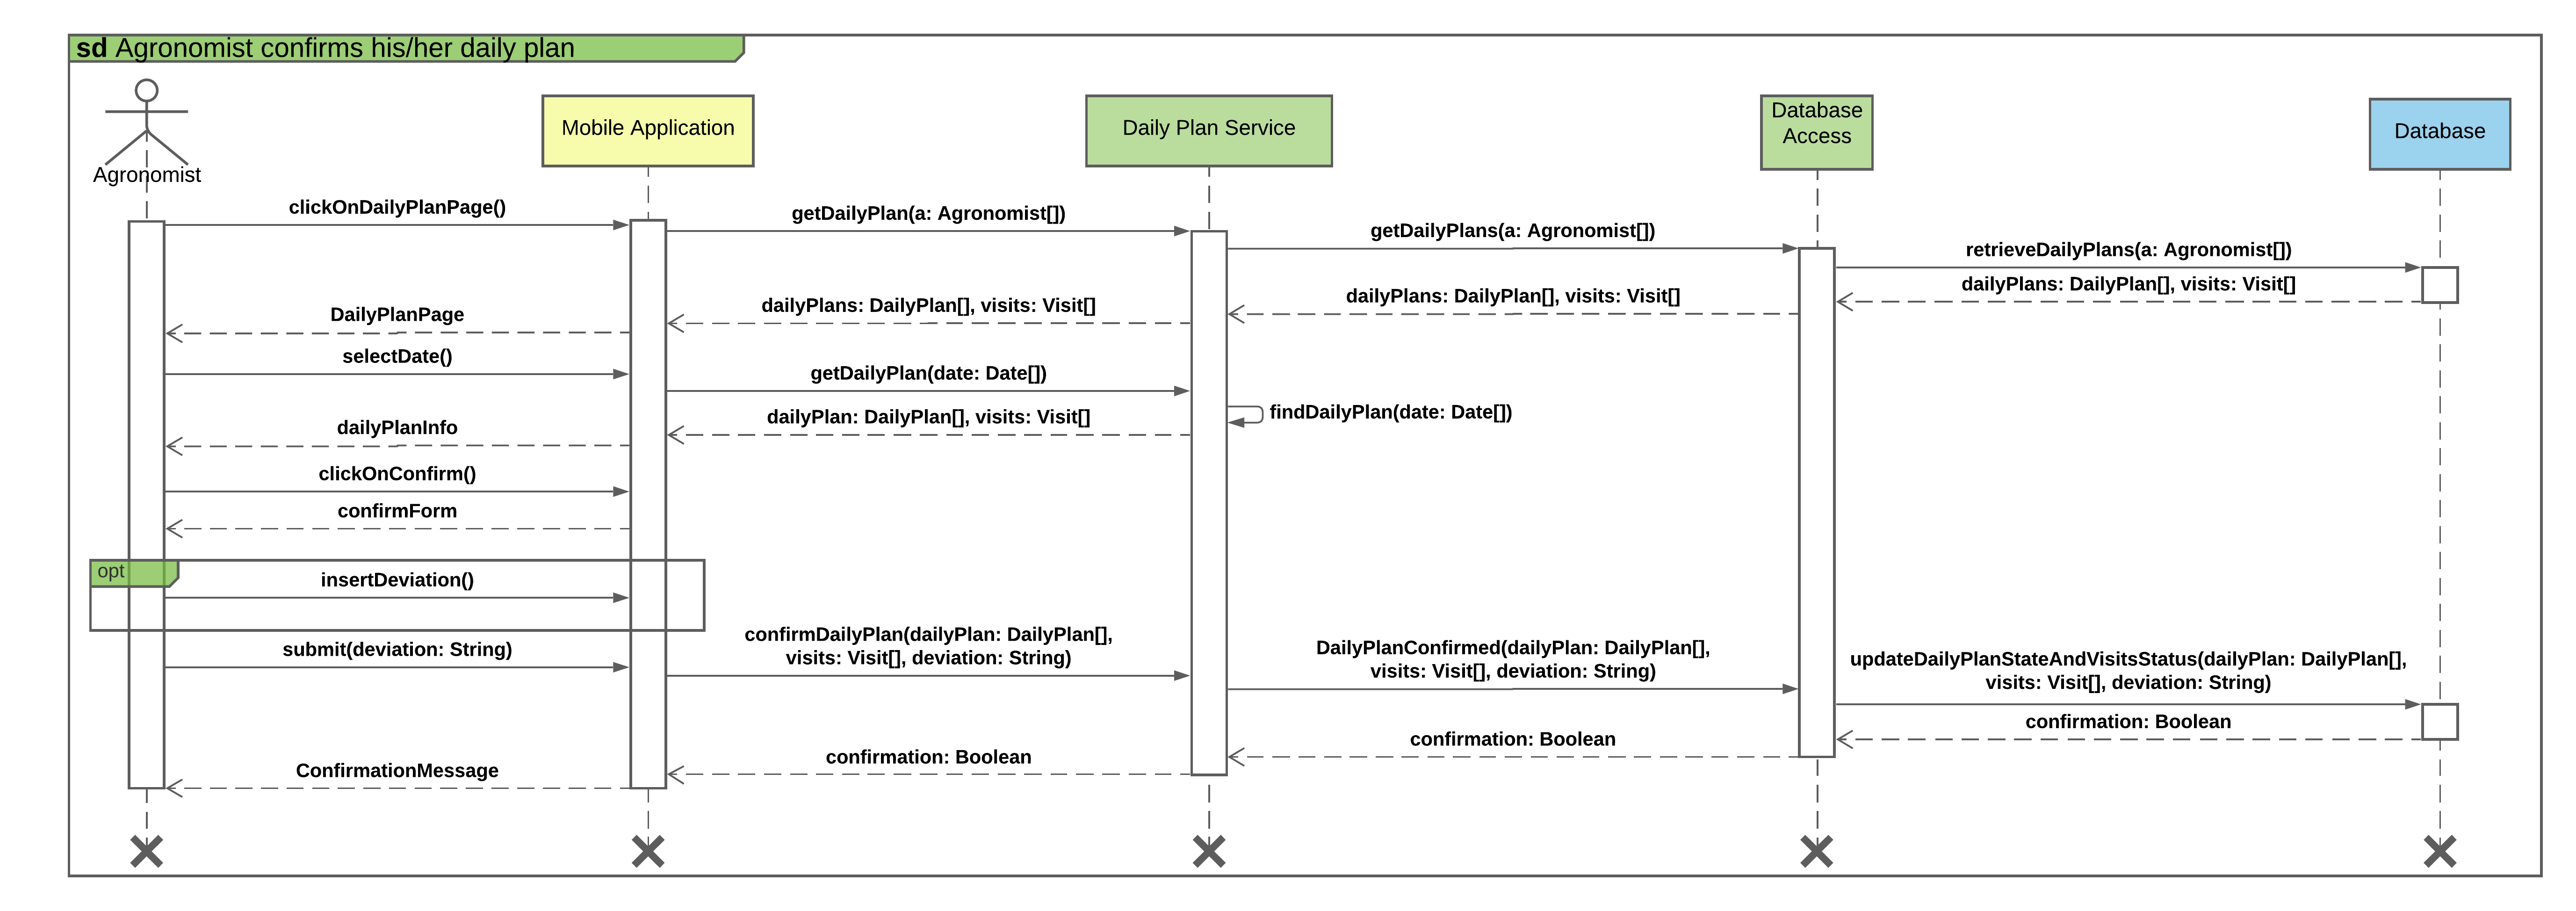
\includegraphics[scale= 0.108]{./Images/Sequence diagram/Agronomist confirms his_her daily plan.png}}
    \caption{Agronomist confirms his/her daily plan}
    \vspace*{-12cm}
\end{figure}
\fillandplacepagenumber
\end{landscape}

\subsection{Policy Maker visualizes and analyzes farmers' data}

This sequence diagram shows the procedure of a policy maker, already registered and logged in, visualizing and analyzing farmers' data in the homepage of the application.\\
The policy maker opens the application and he/she can select map and time chart options. If no option is modified the system process time chart and map automatically with default parameters.  
Web/MobileApplication propagates two requests, one to TimeChartService to get a chart of farmers' performances trend and the other one to MapService to get the Telangana map on which are displayed farmers's performances. For both services is necessary to retrieve from the Database farmers' data(performances and positions). Those data are returned to TimeChartService and to MapService. Both of them compute data according to the parameters selected by the policy maker or those acquired by default, then they return the result. In particular MapService is in charge of processing the map on which will be displayed farmers' performances, to do so it interacts with GoogleMapsAPI external service.
Eventually the \textit{homepage} is shown to the policy maker.

\newpage
\begin{landscape}
\begin{figure}[t!]
\vspace*{1cm}
\noindent
\centering
\centerline{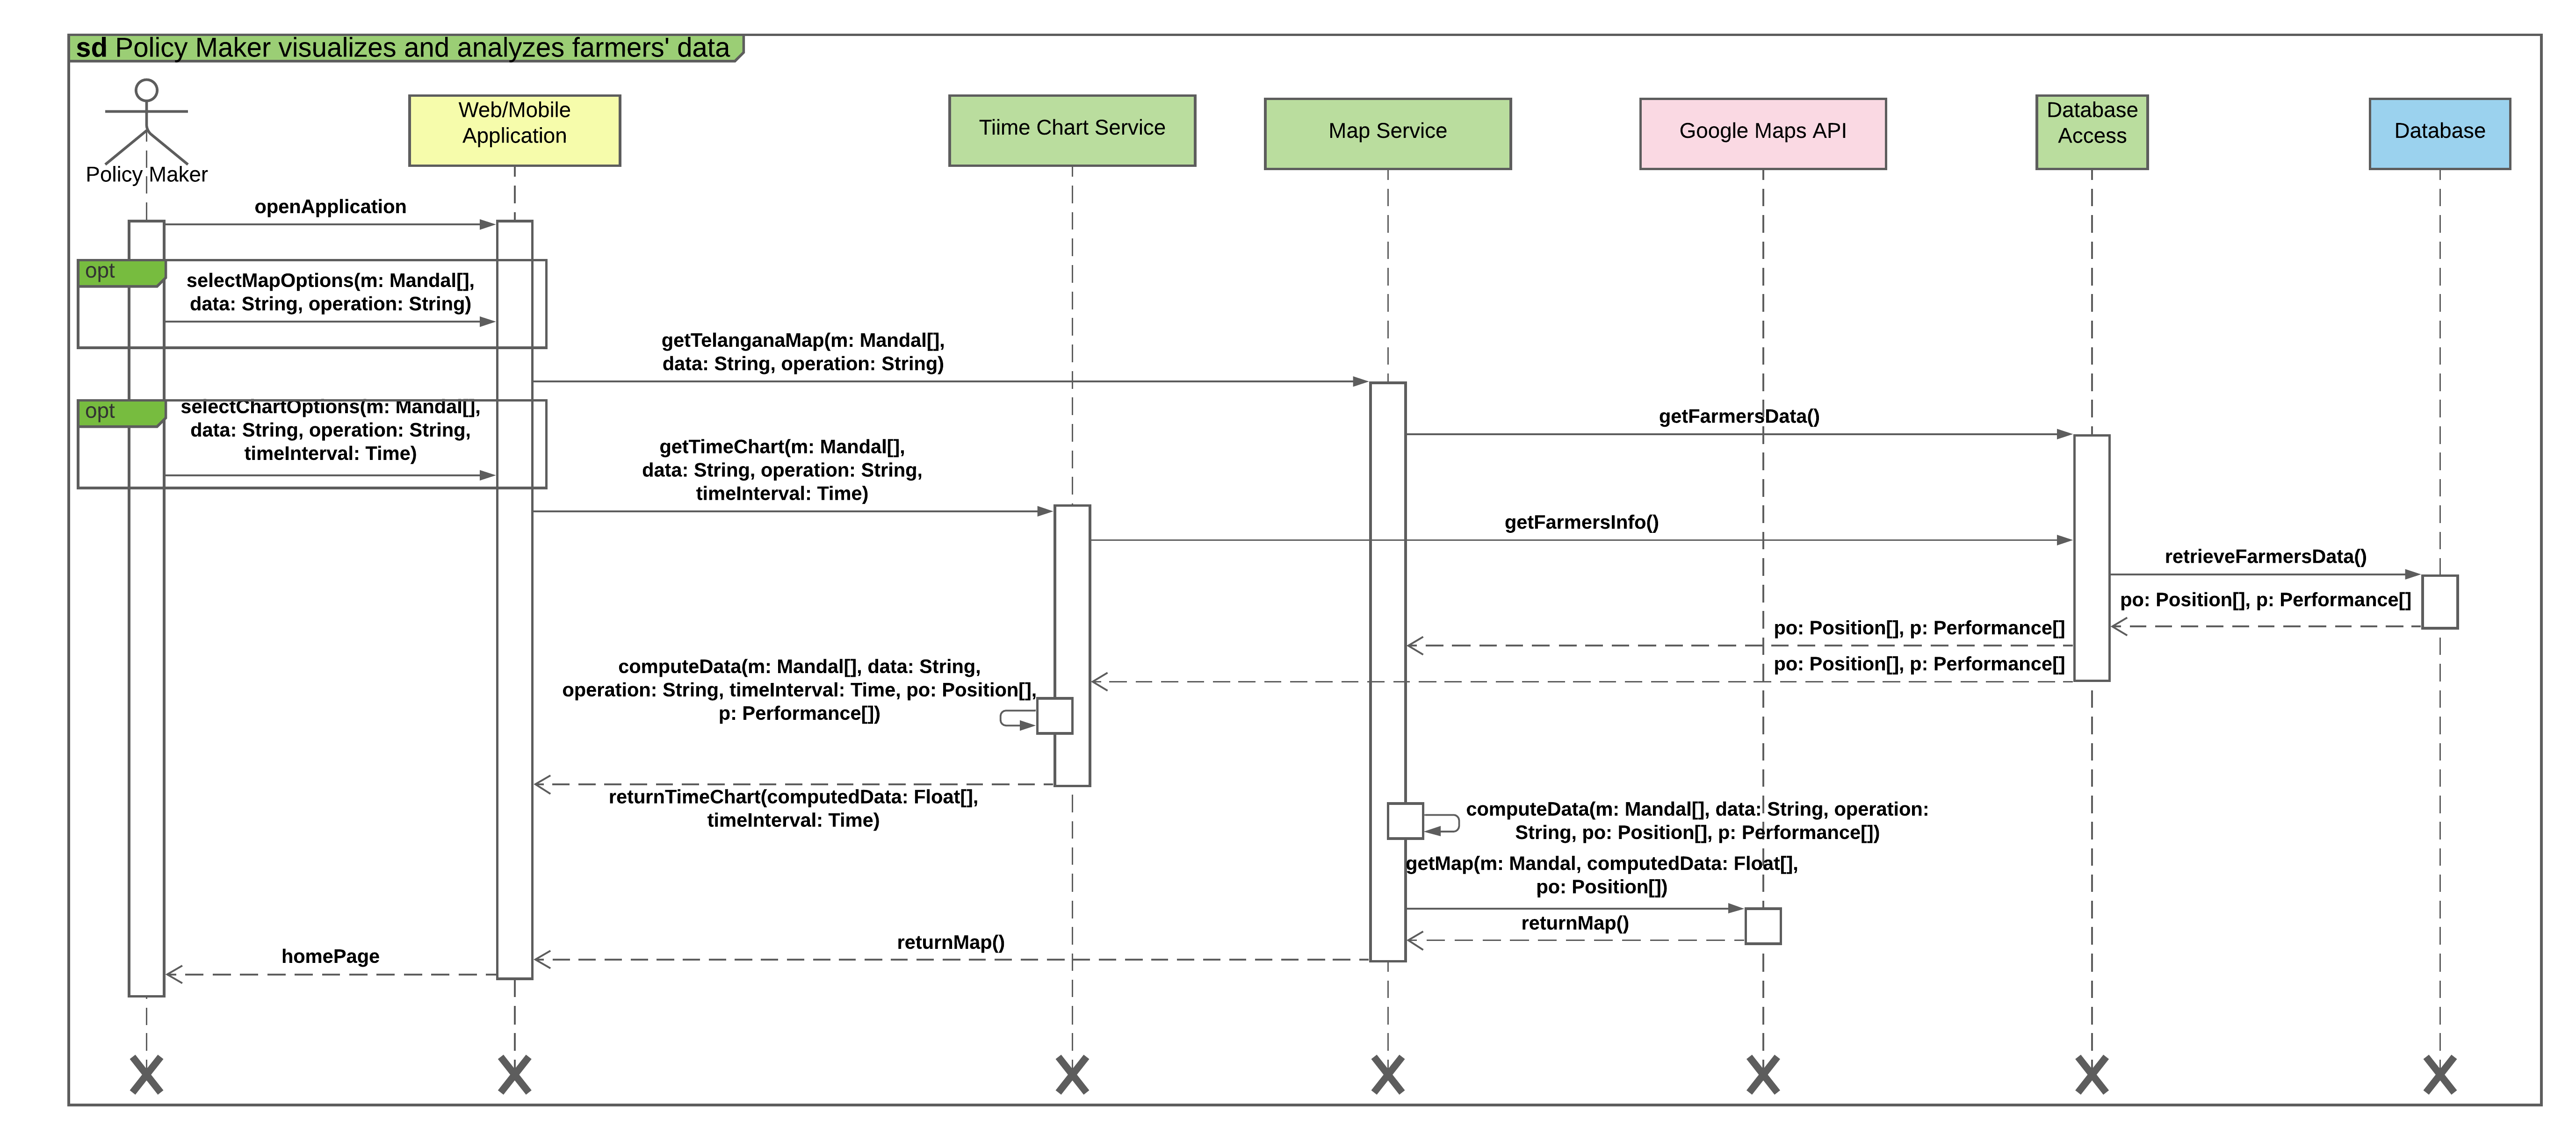
\includegraphics[scale= 0.108]{./Images/Sequence diagram/Policy Maker visualizes and analyzes farmers' data.png}}
    \caption{Policy Maker visualizes and analyzes farmers' data}
    \vspace*{-12cm}
\end{figure}
\fillandplacepagenumber
\end{landscape}


















\section{Component Interfaces}

As shown in \textit{Section 2.4}, many method are invoked on the interfaces. Their interactions guarantee the execution of the most important processes required to fulfill DREAM's goals.\\
The following diagram is presented to better understand how interfaces interact with each other. \\

The methods listed in the previous diagram are a logical representation of what component interfaces have to guarantee the users. \\
Certainly, considering a future implementation, they will be subjected to many modifications, according to choices and needs of developers. 

\section{Selected Architectural Style and Patterns}
This section clarifies the architectural style and architectural pattern adopted in the design of the DREAM system.
The main difference between the two is that an architectural style is the application design at the highest level of abstraction, it is a name given to a recurrent architectural design; while an architectural pattern is a way to implement an architectural style, it is a way to solve a recurring architectural problem related to it.

\subsection{Architectural Style: Client-Server}
In the design of the DREAM application a three tier architecture has been used. It is a client-server architecture in which the functional process logic, data access, computer data storage and user interface are developed and maintained as independent modules on three levels:
\begin{itemize}
    \item a presentation tier;
    \item a logic tier;
    \item a data tier. 
\end{itemize}

In this type of architecture there is the thin client, that is the device that requests the resource, equipped with a user interface in charge of the presentation-level functions. Then, there is the application server, also called middleware, in charge of providing the resource and communicating with the server database, which stores the data used by the application.

The main advantage of the three-tier architecture is the logical and physical separation of functionality. This allows each tier to run on a separate operating system and server platform that best suit its functional requirements.

Compared to one or two tier architecture, this allows for \textbf{faster development} as each tier can be developed simultaneously by several teams. Furthermore, this separation of levels allows programmers to use the latest and best languages and tools for each level.

Moreover, any tier can be scaled independently of the others as needed and if one tier is interrupted, it will be less likely to impact the availability or performance of the other tiers, so this architecture also has a positive impact on \textbf{scalability} and \textbf{reliability} as well.

Since the presentation layer and the data layer cannot communicate directly, a well-designed application layer can function as a kind of internal firewall, preventing some malicious attacks and ensuring \textbf{greater security}.

\subsection{Architectural Pattern: Model-View-Controller Structure}
DREAM application can be structured with the Model-View-Controller (MVC) pattern.
The MVC structure consists of three building blocks: model, view, and controller.
\begin{itemize}
    \item the \textbf{Model} provides the methods to access the data useful for the application;
    \item the \textbf{View} displays the real user interface for the presentation of the data contained in the model and deals with the interaction with users;
    \item the \textbf{Controller} receives the user's commands through the view and implements them by accessing the Model and defining the corresponding View to be presented
\end{itemize}

\begin{figure}[H]
  \centering
  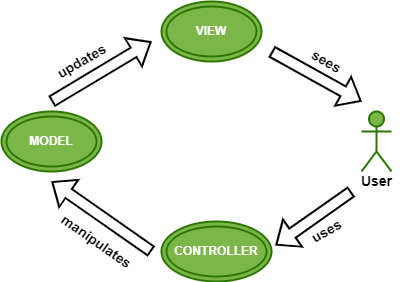
\includegraphics[scale=0.7]{./Images/MVC.png}
  \caption{Model-View-Controller structure}
\end{figure}

This pattern was chosen primarily because application development becomes fast. In fact, it is easier for multiple developers to collaborate and work together given the nature of the architecture itself.
As a result, it also becomes easier to update the application and debug as we have multiple levels properly written in the application.
\section{Other Design Decisions}